\documentclass[russian,10pt]{article}

\usepackage[intlimits]{amsmath}
\usepackage{amsthm,amsfonts}
\usepackage{amssymb}
\usepackage{mathrsfs}
\usepackage{graphicx}
\usepackage{longtable}
\usepackage{indentfirst}
\usepackage[utf8]{inputenc}
\usepackage[T2A]{fontenc}
\usepackage[russian,english]{babel}


\pdfpagewidth 14cm
\pdfpageheight 20cm

\textwidth 11cm
\textheight 16.5cm
\oddsidemargin 1.5cm % 1.84cm
\topmargin 1.5cm % 1.8cm
\footskip 1cm

\hoffset -1in
\voffset -1in
\headheight 0pt
\headsep 0pt

\hyphenpenalty=200
\tolerance=800

% Adjust first page number according to real document position in the book.
\setcounter{page}{1}

% Dot after section number
\makeatletter
% In section title
\def\@seccntformat#1{\csname the#1\endcsname.\quad}
\makeatother

%\tolerance = 2000

% To place author above title
\def\maketitle{
  \begin{center}
Title
  \end{center}
}

\renewcommand{\refname}{Литература}

\date{}

%\sloppy
%\DeclareGraphicsRule{*}{eps}{*}{}
\DeclareMathOperator{\diam}{diam}

\graphicspath{{images/}}
\newcommand{\imgh}[3]{\begin{figure}[!h]\center{\includegraphics[width=#1]{#2}}\caption{#3}\label{Fig:#2}\end{figure}}

% Perfectly typesetted tilde for url links.
%\def\urltilde{\kern -.15em\lower .7ex\hbox{\~{}}\kern .04em}

\addto{\captionsrussian}{
	\renewcommand{\proofname}{\bf Решение. }
}

\usepackage{wasysym}

\theoremstyle{definition}
%\newtheorem{problem}{\noindent\normalsize\bfЗадача \No\!\!}
\newtheorem{problem}{\noindent\normalsize\bf{}}[section]
\renewcommand{\theproblem}{\arabic{problem}}
\newtheorem{example}{\noindent\normalsize\bf{}Пример}
\newtheorem*{definition}{\noindent\normalsize\bf{}Определение}
\newtheorem*{remark}{\noindent\normalsize\bf{}Замечание}
\newtheorem{theorem}{\noindent\normalsize\bf{}Теорема}
\newtheorem{fixme}{\noindent\normalsize\bf{}\frownie{} fixme}
\renewcommand{\thefixme}{}

\newtheorem*{ordre}{\noindent\normalsize\bf{}Указание}

\newenvironment{solution}{\ \begin{proof}\vspace{1em}} {\end{proof} \vspace{2em}}

\newenvironment{comment}{}{}

\newcommand{\rg}{\ensuremath{\mathrm{rg}}}
\newcommand{\grad}{\ensuremath{\mathrm{grad}}}
\newcommand{\diag}{\ensuremath{\mathrm{diag}}}
\newcommand{\const}{\ensuremath{\mathop{\mathrm{const}}}\nolimits}
\newcommand{\Var}{\ensuremath{\mathop{\mathrm{Var}}}\nolimits}
\newcommand{\Exp}{\ensuremath{\mathrm{{\mathbb E}}}}
\newcommand{\Be}{\ensuremath{\mathrm{Be}}}
\newcommand{\Po}{\ensuremath{\mathrm{Po}}}
\newcommand{\Bi}{\ensuremath{\mathrm{Bi}}}
\newcommand{\Ker}{\ensuremath{\mathrm{Ker}}}
\newcommand{\Real}{\ensuremath{\mathrm{Re}}}
\newcommand{\Lin}{\ensuremath{\mathrm{Lin}}}
\newcommand{\Gl}{\ensuremath{\mathrm{Gl}}}
\newcommand{\mes}{\ensuremath{\mathrm{mes}}}
\newcommand{\cov}{\ensuremath{\mathrm{cov}}}


\begin{document}

\selectlanguage{russian}

\maketitle

\tableofcontents


\section{Стандартные задачи}

\begin{problem}
Ребенок играет с десятью буквами разрезной азбуки: А, А, А, Е, И, К, М, М, Т, Т. 
Какова вероятность того, что при случайном расположении букв в ряд он получит слово <<МАТЕМАТИКА>>? 
\end{problem}



\section{Производящие и характеристические функции}

\begin{problem}
Пусть $g(t)$ является характеристической функцией абсолютно непрерывной случайной величины. Являются ли $Re[g]$ и $Im[g]$ характеристическими функциями?
\end{problem}


\section{Законы больших чисел и предельные теоремы}

\begin{problem}
Пусть случайная величина $X_n$ принимает значения 
$2^n$ и $-2^n$ с вероятностями $1/2$. Выполняется ли для последовательности независимых случайных величин 
$X_1$, $X_2$, $\ldots$ закон больших чисел? 
\end{problem}

\begin{ordre}
Покажите, что усредненная сумма последовательности не сходится по вероятности к своему математическому ожиданию, зафиксировав знаки последних двух слагаемых. 
\end{ordre}


\begin{problem}
Пусть случайная величина $X_n$ принимает значения 
$n$, $0$ и $-n$ с вероятностями $1/4$, $1/2$, $1/4$. Выполняется ли для последовательности независимых случайных величин 
$X_1$, $X_2$, $\ldots$ закон больших чисел? 
\end{problem}

\begin{ordre}
 
$$
S_n\xrightarrow{p}0 \,\Leftrightarrow\, S_n\xrightarrow{D}0 \,\Leftrightarrow\, \varphi_{S_n}(t)
\xrightarrow{n\to\infty}1 , 
$$

где $S_n=\frac{X_1+\ldots +X_n}{n}$

\end{ordre}


\begin{problem}
Пусть $\{ X_n\}_{n=1}^{\infty}$ -- последовательность независимых случайных величин, причем $X_n$ принимает значения 
$-\sqrt{n}$, $\sqrt{n}$ с вероятностями $1/2$ каждое. 
Выполняется для этой последовательности закон больших чисел? 
\end{problem}


\begin{problem}
При каких значениях $\alpha > 0$ к последовательности независимых случайных величин $\{ X_n\}_{n=1}^{\infty}$, 
таких что ${\mathbb P}\{ X_n=n^{\alpha}\}={\mathbb P}\{ X_n=-n^{\alpha}\}=1/2$, применим закон больших чисел? 
\end{problem}

\begin{ordre}
Докажите достаточное условие выполнения ЗБЧ:
 \[
Var S_n \xrightarrow {n\to\infty}0
\] 
\end{ordre}


\begin{problem}
Пусть $\{ X_n\}_{n=1}^{\infty}$ --- последовательность случайных величин с дисперсиями $\sigma_i^2$. Доказать, что если все 
корреляционные моменты (ковариации) $R_{ij}$ случайных величин $X_i$ и $X_j$ неположительны и при $n\to\infty$ 
$\frac{\sum\limits_{i=1}^{n} \sigma_i^2}{n^2}\to 0$, то для последовательности $\{ X_n\}_{n=1}^{\infty}$ выполняется закон больших чисел. 
\end{problem}

\begin{problem}
Пусть $\{ X_n\}_{n=1}^{\infty}$ --- последовательность случайных величин с равномерно ограниченными дисперсиями, причем каждая 
случайная величина $X_n$ зависит только от $X_{n-1}$ и $X_{n+1}$, но не зависит от остальных $X_i$. Доказать выполнение для этой 
последовательности закона больших чисел.
\end{problem}


\begin{problem}
Пусть при любом $\lambda >0$ с.в. $\xi _{\lambda } $ имеет распределение Пуассона. Докажите, что $\frac{\xi _{\lambda } -\lambda }{\sqrt{\lambda } } $ слабо сходится (по распределению) к стандартному нормальному распределению при $\lambda \to \infty $.

\begin{ordre}
 Используйте аппарат характеристических функций и теорему о непрерывном соответствии (о том, что слабая сходимость эквивалентна равномерной сходимости соответствующих характеристических функций).
 \end{ordre}
\end{problem}

\begin{problem}

Рассмотрим простую и классическую схему блуждания точки по прямой, соответствующую правилам игры в орлянку:
\[\eta (0)=0,\] 
\[\eta (t+1)=\left\{\begin{array}{cc} {\eta (t)+1,} & {p={1\mathord{\left/ {\vphantom {1 2}} \right. \kern-\nulldelimiterspace} 2} } \\ {\eta (t)-1,} & {p={1\mathord{\left/ {\vphantom {1 2}} \right. \kern-\nulldelimiterspace} 2} } \end{array}\right. .\] 
Занумеруем в порядке возрастания все моменты времени, когда $\eta (t)=0$. Получим с вероятностью 1 бесконечную последовательность $0=\tau _{0} <\tau _{1} <\tau _{2} <...$ Рассмотрим разности $\xi _{i} =\tau _{i} -\tau _{i-1} $, $i=1,2,...$ -- последовательность независимых одинаково распределенных с.в.

\textbf{а)} Найдите распределение $\xi _{i} =\tau _{i} -\tau _{i-1} $, т.е. $P\left\{\xi _{i} =2m\right\}$

\textbf{б)} Покажите, что математическое ожидание с.в. $\xi _{i} =\tau _{i} -\tau _{i-1} $ равно бесконечности. Этот результат можно проинтерпретировать так: среднее время до первого возвращения блуждания в 0 бесконечно.

Тем не менее суммы $\tau _{n} =\sum _{i=1}^{n}\xi _{i}  $ при надлежащей нормировке подчинены предельному распределению: 
\[\mathop{\lim }\limits_{n\to \infty } P\left\{\frac{2\tau _{n} }{\pi n^{2} } <z\right\}=\left\{\begin{array}{cc} {\frac{1}{\sqrt{2\pi } } \int _{0}^{z}e^{-\frac{1}{2x} } x^{-\frac{3}{2} }  dx,} & {z>0} \\ {0,} & {z<0} \end{array}\right. .\] 
Из теоремы о каноническом представлении устойчивых законов (см. лекции,\textbf{ теорема Леви-Хинчина}): Для того чтобы функция распределения была устойчивой, необходимо и достаточно, чтобы логарифм ее характеристической функции представлялся формулой:
\[\ln \varphi (t)=i\gamma t-c|t|^{\alpha } \left(1+i\beta \frac{t}{|t|} \omega (t,\alpha )\right),\] 
где $\gamma $ -- любое действительное число, $-1\le \beta \le 1$, $0<\alpha \le 2$, $c\ge 0$ и
\[\omega (t,\alpha )=\left\{\begin{array}{cc} {tg\left(\frac{\pi }{2} \alpha \right),} & {\alpha \ne 1,} \\ {\frac{2}{\pi } \ln |t|,} & {\alpha =1} \end{array}\right. ,\] 
следует, что такое распределение соответствует каноническому представлению с $\alpha ={1\mathord{\left/ {\vphantom {1 2}} \right. \kern-\nulldelimiterspace} 2} $, $\beta =1$, $\gamma =0$, $c=1$, и принадлежит семейству кривых Пирсона (показано Н. В. Смирновым).

\end{problem}

\begin{problem}
Bывод распределения Хольцмарка: Рассмотрим шар радиуса $r$ с центром в начале координат и $n$ звезд (точек), расположенных в нем наудачу и независимо друг от друга. Пусть каждая звезда имеет единичную массу. Обозначим $X_{1} ,...,X_{n} $ x-компоненты гравитационных сил, соответствующие отдельным звездам, и положим $S_{n} =X_{1} +...+X_{n} $. Устремим $r$ и $n$ к бесконечности так, чтобы $\frac{4}{3} \pi r^{3} n^{-1} \to \lambda $. Показать, что распределение величины $S_{n} $ стремится к симметричному устойчивому распределению с $\alpha ={3\mathord{\left/ {\vphantom {3 2}} \right. \kern-\nulldelimiterspace} 2} $. Можно показать, что задача по существу не изменится, если массу каждой звезды считать с.в. с единичным математическим ожиданием и массы различных звезд предполагать взаимно независимыми с.в. и не зависящими также от их расположения.
\end{problem}

\begin{problem}
Напомним определение сходимости по распределению (частный случай слабой сходимости): $\xi _{n} \mathop{\to }\limits_{}^{d} \xi $ - для любого $x$, такого что функция $F_{\xi } (x)$ непрерывна в точке $x$, имеет место сходимость функций распределения: $F_{\xi _{n} } (x)\to F_{\xi } (x)$ при $n\to \infty $, где $F_{\xi } (x)$ - функция распределения с.в. $\xi $.

\noindent \textbf{а)} Объясните, почему нет слабой сходимости такой последовательности с.в.:
\[\xi _{n} =\left\{\begin{array}{cc} {-n,} & {{\raise0.7ex\hbox{$ 1 $}\!\mathord{\left/ {\vphantom {1 2}} \right. \kern-\nulldelimiterspace}\!\lower0.7ex\hbox{$ 2 $}} ,} \\ {n,} & {{\raise0.7ex\hbox{$ 1 $}\!\mathord{\left/ {\vphantom {1 2}} \right. \kern-\nulldelimiterspace}\!\lower0.7ex\hbox{$ 2 $}} ;} \end{array}\right. \] 

\begin{ordre} 

\noindent $F_{\xi _{n} } (x)=\left\{\begin{array}{cc} {0,} & {x\le -n} \\ {{\raise0.7ex\hbox{$ 1 $}\!\mathord{\left/ {\vphantom {1 2}} \right. \kern-\nulldelimiterspace}\!\lower0.7ex\hbox{$ 2 $}} ,} & {-n<x\le n} \\ {1,} & {x>n} \end{array}\right. $ сходятся к функции $G(x)\equiv \frac{1}{2} $.

\end{ordre} 

\noindent \textbf{б)} Пусть $\xi _{1} ,\xi _{2} ,\xi _{3} ,...$ - последовательность независимых одинаково распределенных с.в. с конечной ненулевой дисперсией. Обозначим $S_{n} =\sum _{i=1}^{n}\xi _{i}  $. При каких значениях $c$ имеет или не имеет место сходимость $P\left(\frac{S_{n} }{n} <c\right)\to P\left(E\xi _{1} <c\right)$?


\end{problem}

\begin{problem}

Доказать локальную предельную теорему:

\noindent Пусть $0<p<1$ и $X_{i} $, $i=1,...,n$ - независимые случайные величины, имеющие распределение:
\[X_{i} =\left\{\begin{array}{cc} {1,} & {p,} \\ {-1,} & {q=1-p;} \end{array}\right. \] 
Тогда равномерно по всем $x=O\left(\sqrt{n} \right)$ таким, что $(p-q)n+x$ целое неотрицательное число
\[P\left\{\sum _{i=1}^{n}X_{i} =(p-q)n+x \right\}\sim \frac{1}{\sqrt{2\pi npq} } \exp \left\{-\frac{x^{2} }{2npq} \right\}\] 
при $n\to \infty $. 

\begin{ordre}
Воспользоваться формулой Стирлинга
\[
n! \sim \sqrt{2 \pi n} \frac{n^n}{e^n} 
\]
\end{ordre}

\begin{remark}
Пусть $n=2k$ и $p=\frac{1}{2} $, тогда вероятность того, что число единиц в точности рано числу минус единиц мало (но не экспоненциально мало):
\[P\left\{\sum _{i=1}^{2k}X_{i} =k \right\}\sim \frac{1}{\sqrt{\pi k} } \] 
\end{remark}

\end{problem}

\begin{problem}
Книга объемом $500$ страниц содержит $50$ опечаток. Оценить вероятность того, что на случайно выбранной странице 
имеется не менее трех опечаток. (Использовать нормальное и пуассоновское приближения, сравнить результаты). 
\end{problem}

\begin{problem}
В тесто для выпечки булок с изюмом замешано $N$ изюмин. Всего из данного теста выпечено $K$ булок. Оценить вероятность того, 
что в случайно выбранной булке число изюмин находится в пределах от $a$ до $b$. 
\end{problem}

\begin{problem}
В поселке $N$ жителей, каждый из которых в среднем $n$ раз в месяц ездит в город, выбирая дни поездки независимо от остальных. 
Поезд из поселка в город идет один раз в сутки. Какова должна быть вместимость поезда для того, чтобы он переполнился с вероятностью, 
не превышающей заданного числа $\beta$? 
\end{problem}

\begin{problem}
В игре в рулетку колесо разделено на 38 равных секторов: 18 красных, 18 белых и два сектора (0 и 00) зеленого цвета. Пусть ставка игрока на каждом шаге равна 1\$. Обозначим $X_{i} $ - выигрыш в i-ой игре. Тогда $X_{1} ,X_{2} ,X_{3} ,...$ - независимые с.в., имеющие распределение: 
\[X_{i} =\left\{\begin{array}{cc} {+1,} & {p={\raise0.7ex\hbox{$ 18 $}\!\mathord{\left/ {\vphantom {18 38}} \right. \kern-\nulldelimiterspace}\!\lower0.7ex\hbox{$ 38 $}} ,} \\ {-1,} & {p={\raise0.7ex\hbox{$ 20 $}\!\mathord{\left/ {\vphantom {20 38}} \right. \kern-\nulldelimiterspace}\!\lower0.7ex\hbox{$ 38 $}} ;} \end{array}\right. \] 
Пусть сыграно $n=361=19^{2} $ партий. Оцените с помощью ЦПТ $P\left(\sum _{i=1}^{n}X_{i}  \ge 0\right)$ и с помощью неравенства Берри-Эссена оцените погрешность приближения.
\end{problem}

\begin{problem}
(Петербургский парадокс) $X_{1} ,X_{2} ,X_{3} ,...$ - независимые с.в., имеющие распределение $P\left(X_{i} =2^{k} \right)=2^{-k} $, $k=1,2,3,...$ То есть, если в игре в орлянку $k$ раз выпал «орел», то выигрыш будет $2^{k} $. Справедливой ценой за игру называют математическое ожидание выигрыша. Но здесь $EX_{i} =\infty $, однако, для этого нужно играть бесконечное число раз и иметь бесконечно много денег. Покажите, что $\frac{S_{n} }{n\log _{2} n} \mathop{\to }\limits^{p} 1$ при $n\to \infty $, где $S_{n} =\sum _{k=1}^{n}X_{k}  $. Проинтерпретируйте результат как цена за $n$ игр?

\begin{ordre} 

Пусть для каждого $n$ с.в. $X_{nk} $, $1\le k\le n$ независимы. Пусть также $b_{n} >0$ с $b_{n} \to \infty $ и $\bar{X}_{nk} =X_{nk} {\rm I} \left\{X_{nk} \le b_{n} \right\}$.(где ${\rm I} \left\{...\right\}$ - индикаторная функция). Предположим, что выполняются условия:
\[1) \sum _{k=1}^{n}P\left\{\left|X_{nk} \right|>b_{n} \right\} \mathop{\to }\limits_{n\to \infty } 0\] 
\[2) \frac{\sum _{k=1}^{n}D\bar{X}_{nk}  }{b_{n} ^{2} } \mathop{\to }\limits_{n\to \infty } 0.\] 
Тогда $\frac{\sum _{k=1}^{n}X_{nk}  -\sum _{k=1}^{n}E\bar{X}_{nk}  }{b_{n} } \mathop{\to }\limits^{p} 0$ при $n\to \infty $.

\noindent Для этой теоремы положите $X_{nk} =X_{k} $. В качестве $b_{n} >0$ возьмите $b_{n} =2^{m(n)} $, где $m(n)$ - целое число, которое можно представить в виде $m(n)=\log _{2} n+K(n)$, $K(n)\to \infty $ при $n\to \infty $. Например, если $K(n)\le \log \log n$, то результатом применения теоремы будет $\frac{S_{n} }{n\log _{2} n} \mathop{\to }\limits^{p} 1$ при $n\to \infty $.

\end{ordre} 

\end{problem}

\begin{problem}

Случайная величина (размер выигрыша) принимает значение $2^{k} -1$ с вероятностью $p_{k} =\frac{1}{2^{k} k(k+1)} $ для $k=1,2,3,...$ и значение\textit{ $-1$} с вероятностью $p_{0} =1-\sum _{k=1}^{\infty }p_{k}  $. Проверьте, что математическое ожидание выигрыша равно нулю. Применив теорему из предыдущей задачи, покажите, что для суммарного размера выигрыша за $n$ партий ($S_{n} $) справедливо$\frac{S_{n} }{{\raise0.7ex\hbox{$ n $}\!\mathord{\left/ {\vphantom {n \log _{2} n}} \right. \kern-\nulldelimiterspace}\!\lower0.7ex\hbox{$ \log _{2} n $}} } \mathop{\to }\limits^{p} 1$.

\begin{ordre}  
Положите $b_{n} =2^{m(n)} $,

 где $m(n)=\min \left\{m:\; 2^{-m} \frac{1}{\sqrt{m^{3}}} \le n^{-1} \right\}$
\end{ordre} 

\end{problem}

\begin{problem}

Определение: Распределение $G\left(x\right)$ называется max-устойчивым, если для любых $n=1,2,...$ существуют $a_{n} >0$ и $b_{n} \in {\mathbb R}$, такие что $G^{n} \left(a_{n} x+b_{n} \right)=G\left(x\right)$.


(MAX-устойчивые распределения: Гумбеля, Фреше, Вейбулла). Пусть есть независимые одинаково распределенные с.в. $X_{1} ,...,X_{n} $ с распределением $F\left(x\right)$. Обозначим $X_{\left(n\right)} =\max \left\{X_{1} ,...,X_{n} \right\}$. Распределение такой с.в. $F_{X_{\left(n\right)} } \left(x\right)=\left[F\left(x\right)\right]^{n} $.

\begin{enumerate}
\item  Пусть $\mathop{\lim }\limits_{x\to \infty } e^{\alpha x} \left(1-F\left(x\right)\right)=\beta $, где $\alpha ,\beta >0$ и $x\in {\mathbb R}$. Покажите, что $X_{\left(n\right)} -\frac{1}{\alpha } \ln \left(\beta n\right)\mathop{\to }\limits^{d} \chi $, где $\chi $ имеет распределение Гумбеля: $P\left(\chi \le x\right)=e^{-e^{-\alpha x} } $, $x\in {\mathbb R}$.

\item  Пусть $\mathop{\lim }\limits_{x\to \infty } x^{\alpha } \left(1-F\left(x\right)\right)=\beta $, где $\alpha ,\beta >0$ и $x\in {\mathbb R}_{+} $. Покажите, что $X_{\left(n\right)} \left(\beta n\right)^{-\frac{1}{\alpha } } \mathop{\to }\limits^{d} \eta $, где $\eta $ имеет распределение Фреше: $P\left(\eta \le x\right)=e^{-x^{-\alpha } } $, $x>0$.

\item  Пусть $\mathop{\lim }\limits_{x\to \infty } \left(c-x\right)^{\alpha } \left(1-F\left(x\right)\right)=\beta $, $F\left(c\right)=1$,где $\alpha ,\beta >0$, $c\in {\mathbb R}$ и $x\in {\mathbb R}$. Покажите, что $\left(X_{\left(n\right)} -c\right)\left(\beta n\right)^{\frac{1}{\alpha } } \mathop{\to }\limits^{d} \gamma $, где $\gamma $ имеет распределение Вейбулла: $P\left(\gamma \le x\right)=e^{-(-x)^{-\alpha } } $, $x<0$.

\end{enumerate}

\noindent Покажите, что распределения Гумбеля, Фреше, Вейбулла являются max-устойчивыми.

\begin{remark}
В классе max-устойчивых распределений распределения Гумбеля, Фреше, Вейбулла исчерпывают все возможные типы предельных распределений.
\end{remark}

\end{problem}


\begin{problem}

Пусть есть независимо одинаково распределенные с.в. $X_{1} ,...,X_{n} $ с распределением Коши $\alpha =1$, т.е. $F\left(x\right)=\frac{2}{\pi } \int _{-\infty }^{x}\frac{dy}{1+y^{2} }  $. Воспользовавшись предыдущей задачей, найдите предельное распределение для должным образом нормированных с.в. $X_{\left(n\right)} $.

\end{problem}

\begin{problem}
Пусть $\vec{X}_{n} \in {\mathbb R}^{m} $, $n=1,2,...$ - независимые одинаково распределенные случайные векторы. $M\vec{X}_{n} =\vec{0}$, $M\vec{X}_{n} \vec{X}_{n}^{T} =R$ ($R$ - неотрицательно определенная матрица - по определению, однако, мы дополнительно будем считать, что $R$ - положительно определенная). С помощью аппарата характеристических функций докажите, что тогда для любого борелевского множества $B\subseteq {\mathbb R}^{m} $:
\[\mathop{\lim }\limits_{N\to \infty } P\left(\frac{1}{\sqrt{N} } \sum _{n=1}^{N}\vec{X}_{n}  \in B\right)=\left(\left(2\pi \right)^{m} \det R\right)^{-{1\mathord{\left/ {\vphantom {1 2}} \right. \kern-\nulldelimiterspace} 2} } \int _{B}e^{-\left(\vec{x},R\vec{x}\right)} d\vec{x} .\] 

\end{problem}

\begin{problem}
Докажите, что при $n\to\infty$ 
$$
X_n\xrightarrow{L_2} X \,\Rightarrow\, X_n\xrightarrow{L_1}X \, \Rightarrow\, X_n\xrightarrow{P}X 
\, \Leftarrow\, X_n\xrightarrow{\text{ п.н. }}X , 
$$
$$
X_n\xrightarrow{P}X \, \Rightarrow\, X_n\xrightarrow{d}X . 
$$
С помощью контрпримеров покажите, что никакие другие стрелки импликации в эту схему в общем случае добавить нельзя. 
При каких дополнительных условиях можно утверждать, что 
$$
X_n\xrightarrow{\text{ п.н. }}X  \, \Rightarrow\, X_n\xrightarrow{L_1}X ?
$$
Кроме того, показать, что 
$$
X_n\xrightarrow{P} X \; (n\to\infty) \,\Leftrightarrow\, \rho_P(X_n,X)={\mathbb E}\Bigl( \frac{|X_n-X|}{1+|X_n-X|}\Bigr)
\xrightarrow{n\to\infty} 0 . 
$$
Также показать, что 
$$
X_n \xrightarrow{d}c\quad \Rightarrow \quad X_n \xrightarrow{P}c, \text{ где } c=\const \text{ (не с.в.) }
$$
\end{problem}

\begin{fixme}
To be refactored
\end{fixme}

\begin{solution}
\begin{enumerate}
\item $X_n\xrightarrow{\text{ п.н. }}X \,\Rightarrow\, X_n\xrightarrow{P}X$. 

Это следует из теоремы из функционального анализа: из сходимости почти наверное последовательности измеримых 
функций $\{ X_n\}$ следует сходимость по мере, в частности, по вероятностной мере. 

\item $X_n\xrightarrow{L_1}X \, \Rightarrow\, X_n\xrightarrow{P}X$. 

Это следует из неравенства Маркова: 
$$
{\mathbb P}(|X_n-X|>\varepsilon)\leqslant \frac{{\mathbb E}|X_n-X|}{\varepsilon} . 
$$

\item $X_n\xrightarrow{L_2} X \,\Rightarrow\, X_n\xrightarrow{L_1}X$. 

Это следует из неравенства $\bigl( {\mathbb E}|X_n-X|\bigr)^2 \leqslant {\mathbb E}|X_n-X|^2$, являющееся неравенством Йенсена вида 
$$
g({\mathbb E}Y)\leqslant {\mathbb E}g(Y) 
$$
для выпуклой функции $g(x)=x^2$ при $Y=|X_n-X|$. 

\item $X_n\xrightarrow{P}X \, \Rightarrow\, X_n\xrightarrow{d}X$ . 

Как доказывается в курсе теории вероятности, сходимость по распределению эквивалентна слабой сходимости, поэтому достаточно доказать, что 
для любой ограниченной непрерывной функции $\varphi(\cdot)$ выполняется 
\begin{equation}
\label{WeakConverg}
\lim\limits_{n\to\infty} {\mathbb E}\varphi(X_n)={\mathbb E}\varphi(X) . 
\end{equation}
Имеем 
$$
\forall\varepsilon>0, \quad \lim\limits_{n\to\infty} {\mathbb P}(|X_n-X|>\varepsilon)=0 . 
$$
$$
|{\mathbb E}\varphi(X_n)-{\mathbb E}\varphi(X)|\leqslant {\mathbb E}|\varphi(X_n)-\varphi(X)|=\int\limits_{\Omega} 
|\varphi(X_n(\omega))-\varphi(X(\omega))|\, P(d\omega)=
$$
$$
=\int\limits_{|\varphi(X_n(\omega))-\varphi(X(\omega))|>\varepsilon}\!\!\!\! |\varphi(X_n(\omega))-\varphi(X(\omega))|\, P(d\omega)\, +
\int\limits_{|\varphi(X_n(\omega))-\varphi(X(\omega))|\leqslant\varepsilon}\!\!\!\! |\varphi(X_n(\omega))-\varphi(X(\omega))|\, P(d\omega). 
$$
Из ограниченности $\varphi$ имеем $|\varphi(x)|<C$, $|\varphi(x)-\varphi(y)|<2C$, поэтому 
\begin{multline*}
\int\limits_{\Omega} |\varphi(X_n(\omega))-\varphi(X(\omega))|\, P(d\omega)< 
2C\cdot {\mathbb P}(|X_n-X|>\varepsilon)+\\
+\int\limits_{|\varphi(X_n(\omega))-\varphi(X(\omega))|\leqslant\varepsilon} |\varphi(X_n(\omega))-\varphi(X(\omega))|\, P(d\omega) . 
\end{multline*}
Из непрерывности $\varphi$ следует, что 
$$
\forall\delta>0 \; \exists\varepsilon>0: 
\quad |X_n(\omega)-X(\omega)|\leqslant\varepsilon \; |\varphi(X_n(\omega))-\varphi(X(\omega))|<\delta \;\text{ и }
$$
$$
2C\cdot {\mathbb P}(|X_n-X|>\varepsilon)+
\int\limits_{|\varphi(X_n(\omega))-\varphi(X(\omega))|\leqslant\varepsilon} |\varphi(X_n(\omega))-\varphi(X(\omega))|\, P(d\omega)
<2C\cdot {\mathbb P}(|X_n-X|>\varepsilon)+\delta . 
$$
Из сходимости $X_n\xrightarrow{P}X$ следует, что $\exists N:\; \forall n\geqslant N\,\Rightarrow \, $ 
${\mathbb P}(|X_n-X|>\varepsilon)<\frac{\delta}{2C}$, откуда 
$$
|{\mathbb E}\varphi(X_n)-{\mathbb E}\varphi(X)|<2\delta . 
$$
Свойство $(\ref{WeakConverg})$ доказано. 

\item Из сходимости по распределению не следует сходимость по вероятности. 

Рассматривается вероятностная тройка $(\Omega,\, {\mathcal F},\, {\mathbb P})$, где $\Omega=[0, 1]$, 
${\mathcal F}$ --- $\sigma$-алгебра борелевских множеств из $\Omega$, ${\mathbb P}$ --- мера Лебега. 
Случайные величины $X(\omega)=\omega$ и $Y(\omega)=1-\omega$ имеют одну и ту же функцию распределения 
$$
F_X(x)=F_Y(x)=x\cdot {\mathbb I}_{\{ x\in[0,1]\}} . 
$$
Поэтому последовательность с.в. $X,Y,X,Y,\ldots$ сходится по распределению, т.к. каждый элемент последовательности имеет 
одну и ту же функцию распределения. При этом, очевидно, сходимости по вероятности нет, т.к. например, 
$$
{\mathbb P}(|X-Y|>0.5)=0.5 . 
$$

Также заметим, что из данного примера следует, что из сходимости по распределению не следует сходимость в $L_1$, в $L_2$ 
и почти наверное, поскольку, как уже доказано, каждая из них влечет сходимость по вероятности. 

\item Из сходимости по вероятности не следует сходимость почти наверное. 

Рассматривается та же вероятностная тройка $(\Omega,\, {\mathcal F},\, {\mathbb P})$. 
Рассмотрим в качестве последовательности с.в. серию бегущих импульсов: 
$$
X_1={\mathbb I}_{[0,1/2]},\, X_2={\mathbb I}_{[1/2,1]},\, X_3={\mathbb I}_{[0,1/4]},\, X_4={\mathbb I}_{[1/4,1/2]}, \ldots, 
$$
в общем виде $n=2^k-2+i$ $\Rightarrow\, X_n={\mathbb I}_{[\frac{i-1}{2^k},\frac{i}{2^k}]}$. 

Последовательность $\{ X_n\}$ не сходится ни в одной точке $\omega$, т.к. при сколь угодно больших $n$ с.в. $X_n$ 
равна как $0$, так и $1$. При этом $X_n\xrightarrow{P}X\equiv 0$, т.к. при малых $\varepsilon>0$ 
$$
{\mathbb P}(|X_n-X|>\varepsilon)={\mathbb P}(|X_n|=1)=\frac{1}{2^{[\log n]}}\xrightarrow{n\to\infty} 0 . 
$$

\item Из сходимости в $L_1$ не следует сходимость почти наверное. 

Последовательность $\{ X_n\}$ из предыдущего пункта сходится к $X\equiv 0$ в $L_1$: 
$$
{\mathbb E}|X_n-X|={\mathbb E}X_n=\frac{1}{2^{[\log n]}}\xrightarrow{n\to\infty} 0 , 
$$
но, как отмечалось, не сходится почти наверное. 

\item Пример, когда из сходимости почти наверное не следует сходимость в $L_1$ или в $L_2$. Из данного примера также 
следует, что из сходимости по вероятности не следует сходимость в $L_1$ или в $L_2$. 

Рассматривается та же вероятностная тройка $(\Omega,\, {\mathcal F},\, {\mathbb P})$. Строим последовательность с.в. 
$$
X_n(\omega)=n^2 \cdot {\mathbb I}_{[0,\frac{1}{n}]} . 
$$
Из данной формулы следует, что последовательность $\{ X_n\}$ сходится к нулю почти наверное и по вероятности. Однако 
$$
{\mathbb E}|X_n|=n^2\cdot\frac{1}{n}=n \xrightarrow{n\to\infty} \infty , 
$$
$$
{\mathbb E}|X_n|^2=n^4\cdot\frac{1}{n}=n^3 \xrightarrow{n\to\infty} \infty . 
$$
Поэтому последовательность $\{ X_n\}$ не сходится в $L_1$ и в $L_2$. 

\item Выполнена импликация 
$$
X_n\xrightarrow{\text{ п.н. }}X  \, \Rightarrow\, X_n\xrightarrow{L_1}X , 
$$
т.е. возможен предельный переход под знаком математического ожидания, если семейство с.в. $\{ X_n\}$ является равномерно интегрируемым: 
$$
\sup\limits_n {\mathbb E}\bigl[ |X_n|\cdot {\mathbb I}_{\{ |X_n|>c\}} \bigr]\xrightarrow{c\to +\infty}0 . 
$$

\item Покажем, что 
$$
X_n\xrightarrow{P} X \; (n\to\infty) \,\Leftrightarrow\, \rho_P(X_n,X)={\mathbb E}\Bigl( \frac{|X_n-X|}{1+|X_n-X|}\Bigr)
\xrightarrow{n\to\infty} 0 . 
$$

\underline{Необходимость}. Очевидно, $\frac{|X_n-X|}{1+|X_n-X|}<1$, $\frac{|X_n-X|}{1+|X_n-X|}\leqslant |X_n-X|$. 
Зафиксируем произвольное $\varepsilon>0$. Имеем 
\begin{multline*}
{\mathbb E}\Bigl( \frac{|X_n-X|}{1+|X_n-X|}\Bigr)=\int\limits_{|X_n-X|\leqslant\varepsilon} 
\frac{|X_n(\omega)-X(\omega)|}{1+|X_n(\omega)-X(\omega)|}\, P(d\omega)+\\
+\int\limits_{|X_n-X|>\varepsilon}
\frac{|X_n(\omega)-X(\omega)|}{1+|X_n(\omega)-X(\omega)|}\, P(d\omega)
\leqslant \varepsilon+{\mathbb P}(|X_n-X|>\varepsilon) . 
\end{multline*}
$X_n\xrightarrow{P} X$, поэтому ${\mathbb P}(|X_n-X|>\varepsilon)\xrightarrow{n\to\infty}0$ и при $n>N_{\varepsilon}$: 
$$
{\mathbb E}\Bigl( \frac{|X_n-X|}{1+|X_n-X|}\Bigr) \leqslant \varepsilon+{\mathbb P}(|X_n-X|>\varepsilon)
\leqslant 2\varepsilon . 
$$
Это и означает, что 
$$
{\mathbb E}\Bigl( \frac{|X_n-X|}{1+|X_n-X|}\Bigr)\xrightarrow{n\to\infty} 0 . 
$$

\underline{Достаточность}. 
Доказываем от противного: пусть нет сходимости последовательности $\{ X_n\}$ по вероятности, тогда 
$$
\exists\varepsilon_0>0, \; \delta>0, \text{ т.ч. } \forall N, \,\exists n>N: \; 
{\mathbb P}(|X_n-X|>\varepsilon_0)>\delta . 
$$
Т.к. функция $g(y)=\frac{y}{1+y}$ монотонно возрастает, для таких $n$ получим 
$$
{\mathbb E}\Bigl( \frac{|X_n-X|}{1+|X_n-X|}\Bigr)\geqslant \int\limits_{|X_n-X|>\varepsilon_0} 
\frac{|X_n(\omega)-X(\omega)|}{1+|X_n(\omega)-X(\omega)|}\, P(d\omega) > \delta\cdot\frac{\varepsilon_0}{1+\varepsilon_0} . 
$$
Это противоречит условию ${\mathbb E}\Bigl( \frac{|X_n-X|}{1+|X_n-X|}\Bigr)\xrightarrow{n\to\infty} 0$, 
поэтому исходное предположение неверно, что завершает доказательство. 

\item 
Итак, пусть $X_n\xrightarrow{d}c$, $c=\const$. Это означает, что $\forall \varepsilon>0$, 
$$
{\mathbb P}(|X_n-c|<\varepsilon)\xrightarrow{n\to\infty}{\mathbb P}(|c-c|<\varepsilon)=1 . 
$$
Это по определению и означает, что $X_n\xrightarrow{P}c$ (при $n\to\infty$). 

\end{enumerate}

\end{solution}



\begin{problem}
Пусть $x_1,\ldots,x_n$ --- независимые одинаково распределенные с.в.. Пусть также характеристическая функция с.в. $x_k$ представляется 
в окрестности $t=0$ в виде 
$$
\varphi_{x_k}(t)={\mathbb E}(e^{it x_k})=1+imt+o(t). 
$$
Используя то, что 
$$
S_n \xrightarrow{d}c\quad \Rightarrow \quad S_n \xrightarrow{P}c, \text{ где } c=\const \text{ (не с.в.) }
$$
и 
$$
S_n \xrightarrow{d}S\quad \Leftrightarrow \quad \varphi_{S_n}(t) \to \varphi_S(t), \text{ равномерно по $t$ в окрестности $t=0$ } , 
$$
найдите 
$$
S_n=\frac{1}{n}\sum\limits_{i=1}^{n} x_i \xrightarrow{P} ?
$$
\end{problem}


\begin{problem}
Пусть $x_1, x_2, x_3, \ldots$ --- последовательность независимых одинаково распределенных с.в.. Положим 
$S_n=\sum\limits_{k=1}^{n} x_k$. Покажите, что 

\begin{enumerate}
\item[1)](з.б.ч.) если ${\mathbb E}(|x_k|)<\infty$, то $S_n/n\xrightarrow{P} m$ при $n\to\infty$, где $m={\mathbb E}(x_k)$; 

\item[2)](ц.п.т.) если ${\mathbb E}(x_k^2)<\infty$, то $(S_n-m\cdot n)/\sqrt{n\cdot D}\xrightarrow{d} N(0,1)$ при $n\to\infty$, 
где $D=\Var x_k$. 

\item[3)](задача математической статистики) Предположим, что независимо $n$ раз кидается монетка с вероятностью выпадения орла в каждом 
опыте равной $p$ (точного значения $p$ мы не знаем, а знаем лишь то, что $0.1\leqslant p\leqslant 0.9$), т.е. $x_k\in\Be(p)$. 
Сколько раз нужно кинуть монетку (оцените $p$), чтобы оценка ${\bar p}(x)=\frac{\sum\limits_{k=1}^{n}x_k}{n}$ с вероятностью 
$\gamma\geqslant 0.95$ отличалась от истинного значения $p$ не более, чем на величину $\delta=0.01$? Применить неравенство Чебышева 
и предельную теорему (точность, которую дает ц.п.т., оцените с помощью неравенства Берри – Эссена). Сравнить результаты. 
\end{enumerate}
\end{problem}

\begin{ordre}

Неравенство Берри – Эссена: 
$$
\sup\limits_{x} \Bigl|{\mathbb P}\Bigl(\sum\limits_{k=1}^{n}\frac{x_k-np}{\sigma\sqrt{n}}<x\Bigr)-\Phi(x)\Bigr|\leqslant 
\frac{C_0\mu^3}{\sigma^3\sqrt{n}} . 
$$
Здесь $C_0<0.7056$, $\,\sigma^2=\Var x_k=p(1-p)$, $\Phi(x)=\int\limits_{-\infty}^{x}\tfrac{e^{-\frac{t^2}{2}}}{\sqrt{2\pi}}\, dt$, 
$$
\mu^3={\mathbb E}|x_k-p|^3. 
$$

\end{ordre}


\begin{problem}
Пусть при каждом $n\geqslant 1$ независимые с.в. $x_{1n}, x_{2n},\ldots, x_{nn}$ таковы, что $x_{kn}\in \Be(p_{kn})$, где 
$\max\limits_{1\leqslant k\leqslant n} p_{kn}\xrightarrow{n\to\infty}0$, $\sum\limits_{k=1}^{n}p_{kn}\xrightarrow{n\to\infty}\lambda$. 
Тогда 
\begin{equation}
\label{TPois}
{\mathbb P}(S_n=m)\xrightarrow{n\to\infty} e^{-\lambda}\frac{\lambda^m}{m!}, \quad m=0,1,2,\ldots, \quad 
\text{ где } S_n=\sum\limits_{k=1}^{n} x_{kn} . 
\end{equation}
\end{problem}

\begin{problem}
В течение дня вы играете в казино и участвуете в $N=100$ независимых розыгрышах. В каждом розыгрыше вы выигрываете с вероятностью 
$p=0.01$. Оцените вероятность того, что вам не удастся ни разу выиграть. Оцените вероятности того, что вы выиграете ровно 
один раз и ровно три раза.

Предположим, что вы ходите играть в казино в течении $n=100$ дней (количество розыгрышей в день и вероятность выиграть не менялись). 
Оцените вероятность того, что за эти $100$ дней вы в общей сложности выиграете не менее $100$ раз, не менее $300$ раз. 

\end{problem}



\begin{problem}
Показать, что при бросании симметричной монеты $n$ раз отношение числа выпадений герба к числу выпадений решки почти наверное стремится 
к $1$ при $n\to\infty$, а вероятность того, что число выпадений герба в точности равняется числу выпадений решки, при четном числе 
бросаний, стремится к $0$ при $n\to\infty$. 
\end{problem}



\begin{problem}
Пусть с.в. $x_n\in \Gamma(\lambda,n)$. Покажите, что из ц.п.т. следует 
$$
\frac{x_n-m(\lambda)\cdot n}{\sigma(\lambda)\cdot\sqrt{n}} \xrightarrow{d} N(0,1) \text{ при } n\to\infty . 
$$
Найдите $m(\lambda)$, $\sigma(\lambda)$. 
\end{problem}



\begin{problem}
Пусть $X_n$ --- последовательность независимых с.в., сходящаяся по вероятности к с.в. $X:\; X_n\xrightarrow{P}X$. Докажите, 
что с.в. $X$ вырождена, т.е. $X\equiv x$, где $x$ --- некоторое число. 
\end{problem}

\begin{solution}
\begin{enumerate}
\item
Из курса функционального анализа известно, что из любой сходящейся по мере (в частности, по вероятностной) последовательности 
измеримых функций (в частности, с.в.) можно выделить подпоследовательность, сходящуюся почти всюду (п.н.): 
$$
X_{n_k}\xrightarrow{\text{ п.н. }}X \text{ при } k\to\infty . 
$$
Если ввести $\sigma$-алгебры $\Xi_n^{\infty}=\sigma(X_n, X_{n+1},\ldots)$ и хвостовую $\sigma$-алгебру 
${\mathcal X}=\bigcap\limits_{n=1}^{\infty}\Xi_{n}^{\infty}$, то событие 
$$
A=\{ \omega: \, X=\lim\limits_{k\to\infty} X_{n_k}\in B \} \in {\mathcal X} , 
$$
где $B$ --- некоторое борелевское множество на ${\mathbb R}$. 

\item
Из закона нуля и единицы Колмогорова для всякого разбиения прямой ${\mathbb R}$ на борелевские множества $\{ B_m\}_{m\geqslant 1}$ 
ровно для одного $m=m_0:$ $\quad {\mathbb P}(A_{B_{m_0}})=1$, для остальных $m:\quad {\mathbb P}(A_{B_m})=0$, где 
$$
A_{B_m}=\{ \omega: \, X=\lim\limits_{k\to\infty} X_{n_k}\in B_m \} . 
$$
Рассматривая для определенности $B_m=[m,m+1)$, далее для разбиения $\{ B^2_m\}_{m=1}^N$ множества $B_{m_0}$, 
$\mu(B^2_m)=\frac{1}{N}$, при некотором $m=m_2$ получим ${\mathbb P}(A_{B^2_{m_2}})=1$. 

Рассуждая так же для разбиения множества $B^2_{m_2}$ и так далее, получим систему вложенных стягивающихся отрезков $\{ B_i\}$, 
$\mu(B_i)\xrightarrow{i\to\infty}0$, так что 
$$
{\mathbb P}\bigl(X=\lim\limits_{k\to\infty} X_{n_k}\in B_i \bigr)=1 . 
$$
Отсюда для единственной общей точки $\{ x\}=\bigcap\limits_{i=1}^{\infty}B_i$ получим 
$$
{\mathbb P}\bigl(X=\lim\limits_{k\to\infty} X_{n_k}=x \bigr)=1 , 
$$
т.е. $X=\lim\limits_{k\to\infty} X_{n_k}\equiv x$ --- вырожденная с.в. 

\end{enumerate}
\end{solution}


\begin{problem}
Число $\alpha$ из отрезка $[0, 1]$ назовем нормально приближаемым рациональными числами, если найдутся $c,\varepsilon>0$ такие, что 
при любом натуральном $q$ 
\begin{equation}
\label{BorelKantel}
\min\limits_{p\in {\mathbb Z}} \Bigl|\alpha-\frac{p}{q} \Bigr|\geqslant \frac{c}{q^{2+\varepsilon}} . 
\end{equation}
Используя лемму Бореля-Кантелли, докажите, что множество нормально приближаемых чисел на отрезке $[0, 1]$ имеет Лебегову меру $1$. 

\end{problem}

\begin{problem}
В некотором городе прошел второй тур выборов. Выбор был между двумя кандидатами $A$ и $B$ (графы <<против всех>> на этих выборах не было). 
Сколько человек надо опросить на выходе с избирательных участков, чтобы исходя из ответов можно было определить долю проголосовавших 
за кандидата $A$ с точностью $5\%$ и с вероятностью не меньшей $0.99$. Считайте, что исходя из голосования в первом туре, известно, 
что каждый из кандидатов наберет не меньше $30\%$ голосов избирателей. 
\end{problem}


\begin{problem}
На множестве $n!$ перестановок $n$ различных элементов задано равномерное распределение. Обозначим через $\xi_k$ случайную величину, 
равную числу инверсий, образованных элементом с номером $k$, т.е. равную числу элементов с номерами меньшими чем $k$, 
которые стоят в перестановке правее элемента с номером $k$. Покажите, что 
$$
\frac{\sum\limits_{k=1}^{n}\xi_k -\left.n^2\right/4}{\left.n^{3/2}\right/6}\xrightarrow{d} N(0,1) \quad \text{ при } n\to\infty . 
$$
\end{problem}

\begin{solution}
\begin{enumerate}

\item Введем с.в. $\xi_{k,i}$, $k>i$: 
$$
\xi_{k,i}={\mathcal I}(\text{<<$k$ находится левее числа $i$>>}) . 
$$
Если позициии всех чисел, кроме $k$ и $i$, фиксированы, то в одной из двух расстановок $k$ находится левее числа $i$, поэтому 
${\mathbb E}\xi_{k,i}=\left.1\right/2$. 

При $i<j<k$, если позиции всех чисел, кроме $k$, $i$ и $j$, фиксированы, то в двух из $6$ расстановок число $k$ находится 
левее чисел $i$ и $j$, а в одной расстановке $k$ левее $j$, и $j$ находится левее $i$, отсюда 
${\mathbb E}(\xi_{k,i}\xi_{k,j})=\left.1\right/3$, ${\mathbb E}(\xi_{k,j}\xi_{j,i})=\left.1\right/6$. 

Наконец, если числа $i$, $j$, $k$, $l$ попарно различны, $i<j$, $k<l$, то с.в. $\xi_{j, i}$ и $\xi_{l,k}$ независимы и 
${\mathbb E}(\xi_{j,i}\xi_{l,k})={\mathbb E}\xi_{j,i}\cdot {\mathbb E}\xi_{l,k}=\left.1\right/4$. 

Поскольку по определению 
$$
\xi_k=\xi_{k,1}+\xi_{k,2}+\ldots +\xi_{k,k-1}, 
$$
имеем ${\mathbb E}\xi_k=\left.(k-1)\right/2$. Далее 
$$
{\mathbb E}\xi_k^2={\mathbb E}\xi_{k,1}^2+\ldots+{\mathbb E}\xi_{k,k-1}^2+2\sum\limits_{i<j<k}{\mathbb E}(\xi_{k,i}\xi_{k,j})=
$$
$$
=\frac{k-1}{2}+2\cdot\frac{(k-1)(k-2)}{2}\cdot\frac{1}{3}=\frac{2k^2-3k+1}{6} , 
$$
откуда $\Var \xi_k={\mathbb E}\xi_k^2-\bigl({\mathbb E}\xi_k \bigl)^2=\frac{k^2-1}{12}$. 

Также вычислим при $k>m$
$$
{\mathbb E}\xi_k \xi_m={\mathbb E}(\xi_{k,1}+\xi_{k,2}+\ldots +\xi_{k,k-1})(\xi_{m,1}+\xi_{m,2}+\ldots +\xi_{m,m-1})=
$$
$$
={\mathbb E}\bigl( \xi_{k,1}\xi_{m,1}+\ldots +\xi_{k,m-1}\xi_{m,m-1} \bigr)+{\mathbb E}\xi_{k, m}(\xi_{m,1}+\ldots +\xi_{m,m-1})+
$$
$$
+\sum\limits_{0<i<k, 0<j<m, i\ne j, i\ne m}{\mathbb E}\xi_{k, i}\xi_{m,j}=\frac{m-1}{3}+
\frac{m-1}{6}+\frac{(k-3)(m-1)}{4}=\frac{(k-1)(m-1)}{4}= {\mathbb E}\xi_k \cdot{\mathbb E}\xi_m. 
$$
Это означает, что с.в. $\xi_k$ и $\xi_m$ некоррелированы, $k\ne m$. 

\item Введем с.в. $T_n=\sum\limits_{k=1}^{n}\xi_k$ --- общее число инверсий в перестановке. Имеем 
$$
{\mathbb E}T_n=\sum\limits_{k=1}^{n} {\mathbb E}\xi_k=\sum\limits_{k=1}^{n} \frac{k-1}{2}=
\frac{1}{4} n(n-1)=\frac{n^2}{4}\bigl(1+O(\left.1\right/n)\bigr) . 
$$
Из некоррелированности с.в. $\xi_k$ и $\xi_m$, $k\ne m$, следует
$$
\Var T_n=\sum\limits_{k=1}^{n} \Var \xi_k=
\sum\limits_{k=1}^{n}\frac{k^2-1}{12}=-\frac{n}{12}+\frac{n(n+1)(2n+1)}{12\cdot 6}=\frac{n^3}{36}\bigl(1+O(\left.1\right/n)\bigr) . 
$$

\item 
Для всякой сл.в. $X_k=\xi_k-{\mathbb E}\xi_k$ характеристическая функция имеет вид 
$$
\varphi_{X_k}(t)=1-\frac{t^2 \Var\xi_k}{2}+{\overline o}(t^2)=1-\frac{t^2(k^2-1)}{24}+{\overline o}(t^2) . 
$$
Для сл.в. $Y_n=\frac{T_n-{\mathbb E}T_n}{\sqrt{\Var T_n}}$, исходя из независимости сл.в. 
$\xi_1$, $\ldots$, $\xi_n$ и свойств характеристических функций, получим 
$$
\varphi_{Y_n}(t)=\varphi_{X_1}\Bigl( \frac{t}{\sqrt{\Var T_n}} \Bigr)\cdot\ldots \cdot \varphi_{X_n}\Bigl( \frac{t}{\sqrt{\Var T_n}} \Bigr). 
$$
Поскольку 
$$
\varphi_{X_k}\Bigl( \frac{t}{\sqrt{\Var T_n}} \Bigr)=1-\frac{3(k^2-1) t^2}{2n^3}+{\overline o}\Bigl( \frac{1}{n^3} \Bigr)=
\exp\Bigl( -\frac{3(k^2-1) t^2}{2n^3}+{\overline o}\Bigl( \frac{k^2}{n^3} \Bigr) \Bigr) , 
$$
находим 
$$
\varphi_{Y_n}(t)=\exp\Bigl( -\sum\limits_{k=1}^n \frac{3(k^2-1) t^2}{2n^3}+\sum\limits_{k=1}^n {\overline o}\Bigl( \frac{k^2}{n^3} \Bigr)
\Bigr)=\exp\Bigl( -\frac{t^2}{2}+{\overline o}(1)\Bigr)\xrightarrow{n\to\infty} \exp\Bigl(-\frac{t^2}{2}\Bigr) , 
$$
откуда из предельных свойств для характеристических функций вытекает 
$$
Y_n=\frac{T_n-{\mathbb E}T_n}{\sqrt{\Var T_n}}\xrightarrow{d} N(0,1) , 
$$
что равносильно 
$$\frac{T_n-\left.n^2\right/4}{\left.n^{3/2}\right/6}\xrightarrow{d} N(0,1) . 
$$

% Согласно ц.п.т. для с.в. $T_n$ имеем при $n\to\infty$ 
% $$
% \frac{T_n-{\mathbb E}T_n}{\sqrt{\Var T_n}}=\frac{T_n-\left.n^2(1+O(\left.1\right/n))\right/4}{\left.n^{3/2}(1+O(\left.1\right/n))\right/6}
% \xrightarrow{d} N(0,1) , 
% $$
% откуда вытекает требуемое соотношение 
% $$
% \frac{T_n-\left.n^2\right/4}{\left.n^{3/2}\right/6}\xrightarrow{d} N(0,1) .  
% $$
\end{enumerate}
\end{solution}


\section{Случайные модели графов}

\begin{problem}

На некоторой реке имеется 6 островов, соединенных между собой системой мостов. Во время летнего наводнения часть мостов была разрушена. При этом каждый мост разрушается с вероятностью ${1\mathord{\left/ {\vphantom {1 2}} \right. \kern-\nulldelimiterspace} 2} $, независимо от других мостов. Какова вероятность того, что после наводнения можно будет перейти с одного берега на другой, используя не разрушенные мосты?

\imgh{70mm}{graphs_bridges.pdf}{Схема мостов}

\end{problem}

\begin{problem}

(Модель Эрдёша-Реньи).

 Пусть есть конечное множество (в дальнейшем множество вершин) $V$. $\xi _{vv'} $ - независимые с.в., занумерованные парами $\left\{v,v'\right\}\in V\times V$, $\vert V \vert = N$.
\[\xi _{vv'} =\left\{\begin{array}{cc} {1,} & {p} \\ {0,} & {1-p} \end{array}\right. .\] 
Таким образом, можно задать абстрактный случайный граф на фиксированном множестве вершин. Покажите, что 

\begin{enumerate}
\item  При $p=\frac{1}{N^{1+\varepsilon } } $, $\varepsilon >0$ среднее число не изолированных вершин в случайном графе $o\left(N\right)$.

\item  При $p=\frac{1}{N^{1-\varepsilon } } $, $\varepsilon >0$ с вероятностью близкой к единице ($N \gg 1$) существует связная компонента порядка $N$.
\end{enumerate}



\end{problem}

\begin{problem} 
Рассматривается конфигурация спинов $\omega =\left\{x_{mn} \right\}$ (где $x_{mn} $ - независимые бернуллиевские с.в. с параметром $p$) на двумерной решетке $\left\{(m,n)\right\}\in {\mathbb Z}^{2} $. Вершину $(m,n)$ назовем занятой, если $x_{mn} =1$. Соединим ребром все соседние (находящиеся на расстоянии 1) занятые вершины. Получится случайный граф $G=G\left(\omega \right)$. Назовем кластером графа $G$ максимальное подмножество $A$ вершин решетки такое, что для любых двух $v,v'\in A$ существует связывающий их путь по ребрам графа $G$. Докажите, что существует такое $0<\bar{p}<1$, что при $p<\bar{p}$ все кластеры конечны с вероятностью 1, а при $p>\bar{p}$ с положительной вероятностью есть хотя бы один бесконечный кластер.


\begin{ordre}
Покажите, что при достаточно малых значения $p$ вероятность события, что все кластеры конечны, равна 1. Покажите, что вероятность того, что кластер, содержащий начало координат и имеющий не менее $N$ вершин, не превосходит $\left(Cp\right)^{N} \mathop{\to }\limits_{N\to \infty } 0$, где $C$ - некоторая константа. А значит и событие: бесконечный кластер содержит начало координат - имеет нулевую вероятность.
\end{ordre}

\end{problem}


\begin{problem}
Найти математическое ожидание числа вершин, принадлежащих древесным компонентам.
\begin{ordre}
Число возможных деревьев на $k$ вершинах равно $k^{k-2}$. 
\end{ordre}
\end{problem}

\begin{problem}
Докажите, что количество лесов на $n$~вершинах с $r$~компонентами, каждая из которых содержит ровно по одной вершине из множества $ \{1, \ldots, r\} $, в точности $rn^{n-1-r}$~штук.
\end{problem}

\begin{problem}
Покажите, что число попарно неизоморфных деревьев на $n$ вершинах не меньше, чем $ c_n n^{-2.5} e^n $, где $ c_n \to \frac{1}{\sqrt{2\pi}}$.
\end{problem}

\section{Метод Монте Карло}

\begin{problem}
Вычисление значения интеграла:

 \textbf{а)} Требуется вычислить с заданной точностью $\varepsilon $ и с заданной доверительной вероятностью $\gamma $ абсолютно сходящийся интеграл $J=\int _{\left[0,\; 1\right]^{m} }f\left(\vec{x}\right)d\vec{x} $. Считайте, что $\forall \; \; \vec{x}\in \left[0,\; 1\right]^{m} \to \left|f\left(\vec{x}\right)\right|\le 1$.

\noindent \textbf{Пояснение. }Введем случайный m-вектор $\vec{X}\in R\left(\left[0,\; 1\right]^{m} \right)$ и с.в. $\xi =f\left(\vec{X}\right)$. Тогда $M\xi =\int _{\left[0,\; 1\right]^{m} }f\left(\vec{x}\right)d\vec{x} =J$. Поэтому получаем оценку интеграла $\bar{J}_{n} =\frac{1}{n} \sum _{k=1}^{n}f\left(\vec{x}^{k} \right) $, где $\vec{x}^{k} $, $k=1,...,n$ -- повторная выборка значений случайного вектора $\vec{X}$ (т.е. все $\vec{x}^{k} $, $k=1,...,n$ -- независимы и одинаково распределены: также как и вектор $\vec{X}$). В задаче требуется оценить сверху число $n$ ($n\gg m$), начиная с которого $P\left(\left|J-\bar{J}_{n} \right|\le \varepsilon \right)\ge \gamma $.

\textbf{б) }Решите задачу из п. а) при дополнительном предположении липшецевости функции $f\left(\vec{x}\right)$, разбив единичный куб на $n=N^{m} $ одинаковых кубиков со стороной ${1\mathord{\left/ {\vphantom {1 N}} \right. \kern-\nulldelimiterspace} N} $, и используя оценку $\bar{J}_{n} =\frac{1}{n} \sum _{k=1}^{n}f\left(\vec{x}^{k} \right) $, где $\vec{x}^{k} $ -- имеет равномерное распределение в \textit{k}-м кубике.

\textbf{в) (метод выделения главной части, метод замены меры (метод существенной выборки), метод включения особенности в плотность) }Решите задачу п. а) не предполагая, что $f\left(\vec{x}\right)$ -- ограниченная функция на единичном кубе. Предложите способы уменьшения дисперсии полученной оценки интеграла. Как можно использовать информацию об особенностях функции $f\left(\vec{x}\right)$?

\end{problem}

\begin{problem}
Пусть с.в. $\eta _{1} $, $\eta _{2} $ имеют равномерное распределение на отрезке $\left[0,1\right]$. Докажите, что с.в. $X$ и $Y$: $X=\sqrt{-2\ln \eta _{1} } \cos \left(2\pi \eta _{2} \right)$, $Y=\sqrt{-2\ln \eta _{1} } \sin \left(2\pi \eta _{2} \right)$ -- независимые и одинаково распределенные: стандартно нормально ${\rm {\mathcal N}}\left(0,1\right)$.

\begin{ordre}
Покажите, что
\[f_{XY} (x,y)=\frac{1}{\sqrt{2\pi } } e^{-\frac{x^{2} }{2} } \frac{1}{\sqrt{2\pi } } e^{-\frac{y^{2} }{2} } =\frac{1}{2\pi } e^{-\frac{x^{2} +y^{2} }{2} } .\] 
Перейдите к полярным координатам, не забыв о якобиане замены переменных.
\end{ordre}

\end{problem}

\begin{problem}

Если $X$ -- с.в., имеющая стандартное нормальное распределение, то $X^{-2} $ имеет устойчивую плотность:
\[\frac{1}{\sqrt{2\pi } } e^{-\frac{1}{2x} } x^{-\frac{3}{2} } , x>0.\] 
Используя это, покажите, что если $X$ и $Y$ -- независимые нормально распределенные с.в. с нулевым математическим ожиданием и дисперсиями $\sigma _{1}^{2} $ и $\sigma _{2}^{2} $, то величина $Z=\frac{XY}{\sqrt{X^{2} +Y^{2} } } $ нормально распределена с дисперсией $\sigma _{3}^{2} $, такой, что $\frac{1}{\sigma _{3}^{2} } =\frac{1}{\sigma _{1}^{2} } +\frac{1}{\sigma _{2}^{2} } $ (Л.Шепп).

\end{problem}

\subsection{Генерация случайных величин}

\begin{problem}
Покажите, что если с.в. $\eta $ равномерно распределена на отрезке $\left[0,1\right]$, то с.в. $\xi =F^{-1} \left(\eta \right)$ имеет функцию распределения $F\left(x\right)$. Предполагается, что $F\left(x\right)$ непрерывна и строго монотонна. Как выглядит формула для моделирования с.в. из показательного распределения с функцией распределения $F\left(x\right)=\left(1-e^{-\lambda x} \right)I\left\{x>0\right\}$? (Стандартный способ моделирования с.в. -- метод обратной функции)
\end{problem}

\begin{problem}

Пусть $\xi $ распределена на $\left[0,1\right]$ с плотностью $f_{\xi } (x)$, представимой в виде степенного ряда $\sum _{k=0}^{\infty }a_{k} x^{k}  $ с $a_{k} \ge 0$. Положим $p_{k} ={a_{k} \mathord{\left/ {\vphantom {a_{k}  (k+1)}} \right. \kern-\nulldelimiterspace} (k+1)} $. Тогда $f_{\xi } (x)=\sum _{k=0}^{\infty }p_{k} \cdot (k+1)x^{k}  $. Примените метод суперпозиции для моделирования с.в. $\xi $.

\begin{ordre}
Метод суперпозиции:

\noindent 1) Разыгрывается значение дискретной с.в., принимающей значения $k=0,1,2,...$ с вероятностями $p_{k} $.

\noindent 2) Моделируется с.в. с функцией распределения $F_{k} (x)$ (например, методом обратной функции).

\end{ordre}

\end{problem}

\begin{problem}
(Теорема Бернштейна) 

\textbf{а)} С помощью неравенства Чебышёва установите следующий результат из анализа: 

\[
\forall \; \; f\in C\left[0,1\right]\to \left\| f_{n} -f\right\| _{C\left[0,1\right]} \xrightarrow[{n\to \infty }]{} 0,
\] 

\[
f_{n} \left(x\right)=\sum_{k=0}^{n}f\left(\frac{k}{n} \right) C_{n}^{k} x^{k} \left(1-x\right)^{n-k} 
\]

\textbf{б)} Исходя из предыдущей задачи и п. а) предложите способ генерирования распределения с.в. $\xi $, имеющей плотность $f_{\xi } \left(x\right)$ с финитным носителем, для определенности, пусть носителем будет отрезок $\left[0,1\right]$.
\end{problem}

\begin{problem}
Как с помощью с.в. $\xi $, равномерно распределенной на отрезке $\left[0,1\right]$ ($\xi \in R\left[0;1\right]$), и симметричной монетки построить с.в. $X$, имеющую плотность распределения $f_{X} (x)=\frac{1}{4} \left(\frac{1}{\sqrt{x} } +\frac{1}{\sqrt{1-x} } \right)$, $x\in \left[0,1\right]$?
\end{problem}

\begin{problem}
(Метод фон Неймана) 

Пусть с.в. $\xi $ распределена на отрезке$\left[a,b\right]$, причем ее плотность распределения ограничена: $\mathop{\max }\limits_{x\in \left[a;b\right]} f_{\xi } (x)=C<\infty $. Пусть с.в. $\eta _{1} $, $\eta _{2} $, \dots  -- независимы и равномерно распределены на $\left[0,1\right]$, $X_{i} =a+\left(b-a\right)\eta _{2i-1} $, $Y_{i} =C\eta _{2i} $, $i=1,2,...$, т.е. пары $\left(X_{i} ,Y_{i} \right)$ независимы и равномерно распределены в прямоугольнике $\left[a,b\right]\times \left[0,C\right]$. Обозначим через $\nu $ номер первой точки с координатами $\left(X_{i} ,Y_{i} \right)$, попавшей под график плотности $f_{\xi } (x)$, т.е. $\nu =\min \left\{i:\quad Y_{i} \le f_{\xi } (X_{i} )\right\}$. Положим $X_{\nu } =\sum _{n=1}^{\infty }X_{n} I\left\{\nu =n\right\} $.

\textbf{а)} Покажите, что с.в. $X_{\nu } $ распределена также как $\xi $.

\textbf{б)} Сколько в среднем точек $\left(X_{i} ,Y_{i} \right)$ потребуется «вбросить» в прямоугольник $\left[a,b\right]\times \left[0,C\right]$ для получения одного значения $\xi $?
\end{problem}

\subsection{Metropolis}

\subsection{Gibbs Sampler}

\subsection{Variational Inference}

\section{Элементы теории информации}

\begin{problem}

Пусть казино делает $n$ бросаний, используя распределение вероятностей на бинарных словах длины $n$ $p\left(x\right)$, где $x=\left\{0,1\right\}^{n} $, известное игроку. При этом казино производит выплаты так, как если бы оно использовало распределении $q\left(x\right)$ (то есть выигранная ставка на 0, после выпадения $x$ исходов увеличивается в $\frac{q\left(x\right)}{q\left(x0\right)} $ раз, выигранная ставка на 1, после выпадения $x$ исходов увеличивается в $\frac{q\left(x\right)}{q\left(x1\right)} $ раз, см. семинар). Докажите, что у игрока есть стратегия, логарифм значения капитала которой равен расстоянию Кульбака-Лейблера $\sum _{x\in \left\{0,1\right\}^{n} }p\left(x\right)\log \frac{p\left(x\right)}{q\left(x\right)}  $ между распределениями $p$ и $q$.

что-то
\end{problem}

\section{Вероятностный метод в комбинаторике}



\section{Вероятностные методы в Computer Science}

\subsection{Рандомизированные алгоритмы}

\begin{comment}
\begin{problem}

Пять философов сидят за круглым столом. В центре стола находится чаша со
спагетти. Между каждой парой соседних философов лежит вилка. Философы чередуют размышления с приемами пищи, не отвлекаясь на второстепенные занятия. Однако
для того, чтобы вытащить спагетти из чаши и донести их до рта философу требуются
две вилки. Каждый философ может взять вилку рядом с ним (если она доступна), или положить - если он уже держит её. Если требуемая вилка занята соседом, голодный философ вынужден ждать - он не может вернуться к размышлениям, не поев. После окончания еды философ кладет обе вилки на стол.

Время одного приема пищи одним философом равномерно распределено на отрезке [0, a]. 
Время одного размышления равномерно распределено на отрезке [0, b].

Данный процесс подвержен взаимной блокировке (Dead Lock): например, если каждый возьмет по левой вилке, то начнется вечное голодание. Для избежания блокировки каждый философ кладет первую вилку, если за время t после ее взятия вторая не освободилась.

Требуется определить распределение времени t, минимизирующее среднее время ожидания после размышления и перед приемом пищи.

\end{problem}
\end{comment}

\begin{problem}
\noindent Алгоритм быстрой сортировки основан на парадигме «разделяй и властвуй». Выбирается из элементов массива опорный элемент, относительно которого переупорядочиваются все остальные элементы. Желательно выбрать опорный элемент близким к значению медианы, чтобы он разбивал список на две примерно равные части. Переупорядочивание элементов относительно опорного, происходит так, что все переставленные элементы, лежащие левее опорного, меньше его, а те, что правее -- больше или равны опорному. Далее процедура быстрой сортировки рекурсивно применяется к левому и правому списку для их упорядочивания по отдельности.

Наихудшие входные данные для описанного алгоритма быстрой сортировки (предполагается, что в качестве опорного элемента выбирается последний элемент обрабатываемого массива) -- элементы уже упорядоченные по возрастанию. 
Откуда следует, что асимптотика времени работы быстрой сортировки в худшем случае $\Theta (n^{2} )$.

Оценить время работы алгоритма быстрой сортировки в среднем. 

\begin{ordre}
Получить рекуррентное соотношение для математического ожидания времени работы, введя индикаторную функцию позиции опорного элемента. 
Воспользоваться соотношением:
\[\begin{array}{l} {\sum _{k=1}^{n-1}k\log k \le \log \frac{n}{2} \sum _{k=1}^{\left\lceil \frac{n}{2} \right\rceil -1}k +\log n\sum _{k=\left\lceil \frac{n}{2} \right\rceil }^{n-1}k =} \\ {=\frac{n(n-1)}{2} \log n-\frac{\left\lceil \frac{n}{2} \right\rceil \left(\left\lceil \frac{n}{2} \right\rceil -1\right)}{2} \le \frac{1}{2} n^{2} \log n-\frac{n^{2} }{8} } \end{array}\] 
 
\end{ordre}

Показать неулучшаемость оценки для произвольного алгоритма сортировки. Привести способ сортировки с асимптотикой $O(n \log n)$ в худшем случае.

\end{problem}


\begin{problem}[Задача поиска k-ой порядковой статистики].

Рекурсивное применение процедуры, основанной на методе быстрой сортировки, позволяет быстро (в среднем) находить k-ую порядковую статистику. Задача вычисления порядковых статистик состоит в следующем: дан список (массив) из $n$ чисел, необходимо найти значение, которое стоит в k-ой позиции в отсортированном в возрастающем порядке списке. 

\noindent Модифицируем алгоритм быстрой сортировки:


 Выбираем опорный элемент. Делим список на две группы. В первой -- элементы меньше опорного, во второй -- больше либо равны.
 Если размер (число элементов) первой группы больше либо равен k, то к ней снова применяется эта процедура. Иначе -- вызывается процедура для второй группы.
 
\noindent Покажите, используя ту же технику, что и при анализе в среднем алгоритма быстрой сортировки, что среднее время работы такого алгоритма линейно.

\begin{ordre}

\noindent Покажите, что выполняется оценка среднего времени работы алгоритма:

\[
E[T(n)]\le E\left\{\sum _{k=1}^{n}X_{k} \left[T\left(\max (k-1,n-k)\right)+O(n)\right] \right\} 
\]
\[ \le \frac{2}{n} \sum _{k=\left\lfloor \frac{n}{2} \right\rfloor }^{n-1}E[T(k)] +O(n)
\]



\end{ordre}
\end{problem}

\begin{remark}

Пусть $a\ge 1$ и $b>1$- константы, $f(n)$ - произвольная функция, $T(n)$ - функция, определенная на множестве неотрицательных целых чисел с помощью рекуррентного соотношения: $T(n)=aT\left(\frac{n}{b} \right)+f(n)$

\noindent где выражение $\frac{n}{b} $интерпретируется либо как $\left\lfloor \frac{n}{b} \right\rfloor $, либо как$\left\lceil \frac{n}{b} \right\rceil $. Тогда асимптотическое поведение функции $T(n)$ можно выразить следующим образом. 

\begin{enumerate}
\item  Если $f(n)=O(n^{\log _{b} a-\varepsilon } )$ для некоторой константы $\varepsilon >0$, то $T(n)=\Theta \left(n^{\log _{b} a} \right)$.

\item  Если $f(n)=\Theta \left(n^{\log _{b} a} \right)$, то $T(n)=\Theta \left(n^{\log _{a} b} \lg n\right)$.

\item  Если $f(n)=\Omega (n^{\log _{b} a+\varepsilon } )$ для некоторой константы $\varepsilon >0$, и для некоторой константы $c<1$ и достаточно больших n выполнено: $af\left(\frac{n}{b} \right)\le cf(n)$, то $T(n)=\Theta \left(f(n)\right)$.
\end{enumerate}

\end{remark}




\begin{problem}

Даны три матрицы $A,B,C$размера $n\times n$. Требуется проверить равенство $AB=C$.

Простой детерминированный алгоритм перемножает матрицы $A$, $B$ и сравнивает результат с $C$. Время работы такого алгоритма при использовании обычного перемножения матриц составляет $O(n^{3} )$, при использовании быстрого - $O(n^{2,376} )$. Вероятностный алгоритм Фрейвалда с односторонней ошибкой проверяет равенство за время $O(n^{2} )$.

Описание вероятностного алгоритма:

\begin{enumerate}
\item \textbf{ }взять случайный вектор $x\in \left\{0,1\right\}^{n} $

\item  вычислить $y=Bx$

\item  вычислить $z=Ay$

\item  вычислить $t=Cx$

\item  если $z=t$ вернуть «да», иначе «нет».
\end{enumerate}

Покажите, что для предъявленного алгоритма выполняется 
\[\begin{array}{l} {P\left\{z=t \vert AB=C\right\}=1,} \\ {P\left\{z \neq t \vert AB\ne C\right\}\ge {\raise0.7ex\hbox{$ 1 $}\!\mathord{\left/ {\vphantom {1 2}} \right. \kern-\nulldelimiterspace}\!\lower0.7ex\hbox{$ 2 $}} .} \end{array}\] 

\begin{ordre} (добавить что надо несколько раз)
Оценить вероятность ошибочного ответа на одной ненулевой строке матрицы $D = AB - C$. 
\end{ordre}

\end{problem}

\begin{comment}

\begin{problem}

Требуется сравнить две битовые строки $a,b$, потребовав как можно меньше информации от обеих строк. Основная идея -- сравнивать не сами строки, а функции от них. Так сравниваются $a\; mod\; p$ и $b\; mod\; p$, для некоторого простого числа $p$. Для этого требуется передать $2\log _{2} p$ бит информации.

Описание алгоритма сравнения строк:

\begin{enumerate}
\item  Пусть $\left|a\right|=\left|b\right|=n$, $N=n^{2} \log _{2} n^{2} $

\item  Выбираем случайное простое число $p$из интервала $\left[2..N\right]$ 

\item  Выдать «да», если $a\; mod\; p=b\; mod\; p\Leftrightarrow (a-b)\equiv 0\; mod\; p$, иначе выдать «нет».
\end{enumerate}

\noindent  Обоснуйте выбор именно простого числа на шаге 2 и предложите способ его генерации.  

\noindent Покажите что,

\[\begin{array}{l} {P\left\{(a-b)\equiv 0,mod(p)|a=b\right\}=1,} \\ {P\left\{(a-b)\equiv 0,mod(p)|a\ne b\right\}=O\left({\raise0.7ex\hbox{$ 1 $}\!\mathord{\left/ {\vphantom {1 n}} \right. \kern-\nulldelimiterspace}\!\lower0.7ex\hbox{$ n $}} \right),} \end{array}\] 
 
При этом необходимое количество переданных бит равно $O\left(\log _{2} n\right)$.

\begin{ordre}

Воспользоваться асимптотическим законом распределения простых чисел:
\[\mathop{\lim }\limits_{n\to \infty } \frac{\pi \left(n\right)}{{\raise0.7ex\hbox{$ n $}\!\mathord{\left/ {\vphantom {n \ln n}} \right. \kern-\nulldelimiterspace}\!\lower0.7ex\hbox{$ \ln n $}} } =1,\] 
где $\pi \left(n\right)$ - функция распределения простых чисел, равная количеству простых чисел, не превосходящих $n$.

\end{ordre}

\end{problem}

\begin{remark} (мелким шрифтом)
В предыдущей задаче потребуется проверка простоты числа. 
Согласно малой теореме Ферма, если $N$ - простое число и целое $a$ не делится на $N$, то  
\[a^{N-1} \equiv 1\; mod\; N                         \; \; \;            \left(*\right)\] 

Отсюда следует, что если при каком-то $a$ сравнение $\left(*\right)$ нарушается, то можно утверждать, что $N$ - составное. 
К сожалению,  простой вариант подбора $a$ не всегда позволяет эффективно выявить составное число. Имеются составные числа $N$, обладающие свойством $\left(*\right)$ для любого целого $a$ с условием $\left(a,N\right)=1$ ($a$ и $N$ - взаимно простые). Такие числа называются числами Кармайкла.

В 1976г. Миллер предложил заменить проверку $\left(*\right)$ проверкой несколько иного условия. Если $N$ - простое число, то $N-1=2^{s} t$, где $t$ нечетно, то согласно малой теоремы Ферма для каждого a с условием $\left(a,N\right)=1$ хотя бы одна из скобок в произведении 
\[\left(a^{t} -1\right)\left(a^{t} +1\right)\left(a^{2t} +1\right)\times \ldots \times \left(a^{2^{s-1} t} +1\right)=a^{N-1} -1\] 
делится на $N$. 

Пусть $N$ - нечетное составное число, $N-1=2^{s} t$, где \textbf{$t$ }нечетно. Назовем целое число $a$, $1<a<N$ «выявляющим» для $N$, если нарушается одно из двух условий:

I) $N$ не делится на $a$

II) $a^{t} \equiv 1\; mod\; N$ или существует целое $k$, $0\le k<s$ такое, что 

$a^{2^{k} t} \equiv -1\; mod\; N$.

Если $N$ составное число, то согласно теореме Рабина  существует не менее $\frac{3}{4} \left(N-1\right)$  выявляющих чисел.

\end{remark}

\begin{problem}

Пусть $f(x_{1} ,...,x_{n} )=C_{1} \vee \cdots \vee C_{m} $ - булева формула в дизъюнктивной нормальной форме (ДНФ), где каждая скобка $C_{i} $ - есть конъюнкция $L_{1} \wedge \cdots \wedge L_{k_{i} } $ $k_{i} $ литералов (литерал есть либо переменная, либо ее отрицание). Набор значений переменных $a=(a_{1} ,...,a_{n} )$ называется выполняющим для $f$, если $f(a_{1} ,...,a_{n} )=1$. Требуется найти число выполняющих наборов для данной ДНФ.

\noindent $V$ - множество всех двоичных наборов длины $n$.

\noindent $G$ - множество выполняющих наборов.


\noindent  Проведем $N$ независимых испытаний:

\noindent Выбираем случайно $v_{i} \in V$ ( в соответствии с равномерным распределением).
\noindent $y_{i} =f(v_{i} )$. Заметим, что $P\left\{y_{i} =1\right\}=\frac{\left|G\right|}{\left|V\right|} =p$.
Рассмотрим сумму независимых случайных величин $Y=\sum _{i=1}^{N}y_{i}  $. В качестве аппроксимации $\left|G\right|$ возьмем величину $\frac{Y}{N} \left|V\right|$.

\noindent Оцените необходимое число испытаний $N$ как функцию от $|V|$, $|G|$ и точности аппроксимации $\varepsilon$. 

\begin{ordre}
Докажите следующее утверждение. Пусть $X_{1} ,...,X_{n} $ - независимые случайные величины, принимающие значения 0 или 1, при этом $P\left\{X_{i} =1\right\}=p,\quad P\left\{X_{i} =0\right\}=1-p$. Тогда для $X=\sum _{i=1}^{N}X_{i}  $ и для любого $0<\delta <1$, выполнены неравенства
\[\begin{array}{l} {P\left\{X>(1+\delta )EX\right\}\le e^{-\frac{\delta ^{2} }{3} EX} } \\ {P\left\{X<(1-\delta )EX\right\}\le e^{-\frac{\delta ^{2} }{2} EX} } \end{array}\] 
\end{ordre}

\end{problem}


\begin{problem}

(Задача о покрытии). Дано конечное множество из m элементов и система его подмножеств $S_{1} ,...,S_{n} $. Требуется найти минимальную по числу подмножеств подсистему $S_{1} ,...,S_{n} $, покрывающую все множество объектов. 

\noindent Сформулируем ее в терминах булевых матриц и целочисленного линейного программирования:
\[\left\{\begin{array}{l} {cx\to \min ,} \\ {Ax\ge b,} \\ {\forall j\; x_{j} \in \{ 0,1\} .} \end{array}\right. \] 
Здесь переменные $x_{1} ,...,x_{n} $ соответствуют включению подмножеств $S_{1} ,...,S_{n} $ в решение-покрытие, матрица $A$ - матрица инцидентности, $c=(1...1)^{T} \in {\mathbb R}^{n} ,\quad b=(1...1)^{T} \in {\mathbb R}^{m} $ - векторы стоимости и ограничений.

\noindent Пусть элементы матрицы инцидентности -- независимые случайные величины с бернулевским распределением:$P\{ a_{ij} =1\} =p,$ $P\{ a_{ij} =0\} =1-p$. 

\noindent Для решения задачи применяется жадный алгоритм: на каждом шаге выбирается подмножество, максимально покрывающее еще не покрытые объекты. 

Доказать следующее утверждение. Пусть для случайной матрицы $A$, определенной выше, выполнены соотношения:
\[\begin{array}{l} {\forall \gamma >0:} \\ {\frac{\ln n}{m^{\gamma } } \mathop{\to }\limits_{n\to \infty } 0,} \\ {\frac{\ln m}{n} \mathop{\to }\limits_{n\to \infty } 0.} \end{array}\] 
Тогда для $\forall \varepsilon >0:$ $P\left\{\frac{Z}{M} \le 1+\varepsilon \right\}\mathop{\to }\limits_{n\to \infty } 1$, где Z -- решение жадного алгоритма, M -- величина минимального покрытия. 

\begin{fixme}
Добавить указание.
\end{fixme}

\end{problem}

\end{comment}

\begin{problem}
А) Пусть имеется генератор случайных чисел, в 
результате обращения к которому появляется 0 или 1 с одинаковой вероятностью 
равной 1/2 (аналог подбрасывания симметричной монеты). Пусть задано 
вещественное число $0\le p\le 1$. С помощью имеющегося генератора определить 
генератор randp, в результате обращения к которому появляется 0 или 1 с 
вероятностями $p$ и $1-p$ соответственно (незначительные отклонения 
допустимы). Оцените сложность в среднем алгоритма получения одного 
случайного числа с помощью randp (затраты определяются числом обращений к 
изначально имеющемуся генератору). 

Б) Пусть имеется генератор 
случайных чисел randp (описанный выше). Известно, что $p\ne 0,\quad p\ne 1$. 
Как с помощью него сконструировать генератор, в результате обращения 
которому появляется 0 или 1 с одинаковой вероятностью 1/2. 

В) Чему равно математическое ожидание числа обращений к изначально имеющемуся 
генератору случайных чисел при построении последовательности пар до 
появления 0,1 или 1,0? Найти сложность в среднем алгоритма получения k 
``равновероятных'' нулей и единиц с помощью сконструированного генератора 
(затраты определяются количеством обращений к изначально имеющемуся 
генератору). Можно ли указать значения $p$, для которых эта сложность имеет 
минимальное и, соответственно, максимальное значение?
\end{problem}


\begin{problem}[интерактивные доказательства]. 

А) (изоморфизм графов). Алисе известен изоморфизм $\phi$ графов $G_0$ и $G_1$. Но она посылает Бобу граф $H =\psi(G_0)$, либо $H =\psi(G_1)$, где $\psi$ – некоторый другой изоморфизм, не равный $\phi$. Боб бросает симметричную монетку и просит изоморфизм либо $H : G_0$, либо $H : G_1$. В первом случае Алиса посылает  $\psi$, во втором – $\psi \phi^{-1}$. Таких партий разыгрывается $N$ штук. Заметим, что в каждой новой партии Алиса придумывает новую перестановку $\psi$   вершин графа $G_0$. Если $\phi$  – действительно изоморфизм $G_0 : G_1$, то все проверки Боба будут положительны.
Покажите, что если $\phi$ – блеф, то с вероятностью  $1 - 2^{-N}$  хотя бы одна проверка обнаружит это (та проверка, в которой Боб попросил $H : G_1$).

\begin{remark}
Этот пример поучителен с точки зрения «криптографического фокуса» – Алиса убедила Боба в $G_0 : G_1$ так и не огласив самого изоморфизма $\phi$. Если $\phi$ – пароль, то диалог можно вести даже в открытую, что служит примером криптосистемы с нулевым разглашением.
\end{remark}

Б) (неизоморфизм графов). Теперь наделим Алису сверхъестественными вычислительными способностями. Для удобства переименуем игроков: «Prover» и «Verifier». Verifier выбирает случайно (равновероятно) $ i \in \lbrace 0, 1 \rbrace$ и некоторую перестановку $\pi$ вершин графа $G_i$, затем посылает граф $H =\psi(G_i)$ и требует, чтобы Prover определил $i$. Таких партий разыгрывается $N$ штук. Аналогично предыдущему примеру, $\pi$ в каждой новой партии свое. Если графы неизоморфны, то Prover всегда верно определит индекс $i$. Все тесты будут пройдены. Покажите, что иначе с вероятностью $2^{-N}$  Prover ошибется хотя бы один раз (хотя бы в одной партии).
 
\end{problem}

\begin{problem}[доказательство знаний при их отсутствии].
\end{problem}



\subsection{Теория игр}
\begin{problem}
Один игрок прячет (зажимает в кулаке) одну или две монеты достоинством 10 рублей. Другой игрок должен отгадать сколько денег у первого спрятано. Если отгадывает, то получает деньги, если нет -- платит 15 рублей. Каковы  должны быть стратегии игроков при многократном повторении игры?

\end{problem}


\begin{comment}
\begin{problem}
Некто обладает одной облигацией, которую намеревается продать в один из последующих четырех дней, в которых цена облигации 
принимает различные значения, априори неизвестные, но становящиеся известными в начале каждого дня продаж. Предполагается, что 
цены облигации независимы и их перестановки по торговым дням равновозможны. Какова стратегия продавца, состоящая в выборе дня 
продажи облигации и гарантирующая максимальную вероятность того, что он продаст облигацию в день ее наибольшей цены? 
\end{problem}

\begin{ordre}
Рассмотреть следующие возможные стратегии и сравнить вероятности продажи облигации в день наибольшей цены: 
\begin{enumerate}
\item[а)] на первом шаге (в первый день торгов) запомним имевшую место цену облигации, не продавая ее, а затем продадим 
облигацию в тот день, когда ее цена окажется большей цены, зафиксированной в первый день, или (когда такого дня не окажется) в 
последний (четвертый) день, независимо от цены этого дня (стратегия $S_1$); 

\item[б)] не продавая облигацию в первом и втором торговых днях, зафиксируем  максимальную цену из двух, имевших место для этих дней, 
и продадим облигацию в третьем торговом дне, если цена облигации в нем будет выше, чем указанная зафиксированная максимальная цена, 
или, в противном случае, в четвертом дне (стратегия $S_2$). 
\end{enumerate}
\end{ordre}
\end{comment}

\begin{problem}
Ведущий приносит два одинаковых конверта и говорит, что в них лежат деньги, причем в одном вдвое больше, чем в другом. Двое участников берут конверты и тайком друг от друга смотрят, сколько в них денег. Затем один говорит другому: «Махнемся не глядя?» (предлагая поменяться конвертами). Стоит ли соглашаться?
\end{problem}

\begin{comment}
\begin{problem}[парадокс Монти–Холла ](сократить)
Представьте, что вы стали участником игры, в которой находитесь перед тремя дверями. Ведущий поместил за одной из трех 
пронумерованных дверей автомобиль, а за двумя другими дверями --- по козе (козы тоже пронумерованы) случайным образом --– это значит, 
что все $3! = 6$ вариантов расположения автомобиля и коз за пронумерованными дверями равновероятны). У вас нет никакой информации 
о том, что за какой дверью находится. Ведущий говорит: <<Сначала вы должны выбрать одну из дверей. После этого я открою одну из 
оставшихся дверей (при этом если вы выберете дверь, за которой находится автомобиль, то я с вероятностью $1/2$ выберу дверь, 
за которой находится коза номер $1$, и с вероятностью $1-1/2=1/2$ дверь, за которой находится коза номер $2$). Затем я предложу 
вам изменить свой первоначальный выбор и выбрать оставшуюся закрытую дверь вместо той, которую вы выбрали сначала. Вы можете 
последовать моему совету и выбрать другую дверь, либо подтвердить свой первоначальный выбор. После этого я открою дверь, 
которую вы выбрали, и вы выиграете то, что находится за этой дверью.>> Вы выбираете дверь номер $3$. Ведущий открывает дверь номер $1$ 
и показывает, что за ней находится коза. Затем ведущий предлагает вам выбрать дверь номер $2$. Увеличатся ли ваши шансы 
выиграть автомобиль, если вы последуете его совету? 
\end{problem}


 \begin{problem}
 В аудитории находится невеста, которая хочет выбрать себе жениха. За дверью выстроилась очередь из $N$ женихов. Относительно любых 
 двух женихов невеста может сделать вывод, какой из них для неё предпочтительнее. Таким образом, невеста задает на множестве женихов 
 отношение порядка (естественно считать, что если $A$ предпочтительнее $B$, а $B$ предпочтительнее $C$, то $A$ предпочтительнее $C$). 
 Предположим, что все $N!$ вариантов очередей равновероятны и невеста об этом знает (равно, как и число $N$). Женихи запускаются 
 в аудиторию по очереди. Невеста видит каждого из них в первый раз! Если на каком-то женихе невеста остановится (сделает свой выбор), 
 то оставшаяся очередь расходится. Невеста хочет выбрать наилучшего жениха (исследуя $k$–го по очереди жениха, невеста лишь может 
 сравнить его со всеми предыдущими, которых она уже просмотрела и пропустила). Оцените (при $N\to\infty$) вероятность того, что невесте 
 удастся выбрать наилучшего жениха, если она придерживается следующей стратегии: просмотреть (пропустить) первых по очереди $[N/e]$ 
 кандидатов и затем выбрать первого кандидата, который лучше всех предыдущих (впрочем, такого кандидата может и не оказаться, тогда, 
 очевидно, невеста не смогла выбрать наилучшего жениха). 
 \end{problem}
 
 \end{comment}
 

\begin{problem}
В аудитории находится 100 человек (игроков). Каждого просят написать  число от 1 до 100. Победителем окажется тот участник, который написал число наиболее близкое к $\frac{2}{3}$ от среднего арифметического всех чисел. Найти оптимальную стратегию, при условии, что каждый участник думает на $x \sim Poisson(2)$  хода  вперед.  
\end{problem}

 \begin{comment}
\begin{problem}[сублинейный приближенный вероятностный алгоритм для 
матричных игр; Григориадис -- Хачиян, 1995]
Рассматривается симметричная 
антагонистическая игра двух лиц X и Y. Смешанные стратегии X и Y будем 
обозначать соответственно $\vec {x}$ и $\vec {y}$. При этом $x_k $ - 
вероятность того, что игрок X выберет стратегию с номером k, аналогично 
определяется $y_k $. Таким образом, $\vec {x},\vec {y}\in S=\left\{ {\vec 
{x}\in {\rm R}^n:\;\;\vec {e}^T\vec {x}=1,\;\vec {x}\ge \vec {0}} \right\}$, 
где $\vec {e}=\left( {1,...,1} \right)^T$. Выигрыш игрока X: $V_X \left( 
{\vec {x},\vec {y}} \right)=\vec {y}^TA\vec {x}$, а выигрыш игрока Y: $V_Y 
\left( {\vec {x},\vec {y}} \right)=-\vec {y}^TA\vec {x}$ (игра 
антагонистическая). Каждый игрок стремится максимизировать свой выигрыш, при 
заданном ходе оппонента. Равновесием Нэша (в смешанных стратегиях) 
называется такая пара стратегий $\left( {\vec {x}^\ast ,\;\vec {y}^\ast } 
\right)$, что
\[
\vec {x}^\ast \in \mbox{Arg}\mathop {\max }\limits_{\vec {x}\in S} \vec 
{y}^{\ast T} A\vec {x},
\quad
\vec {y}^\ast \in \mbox{Arg}\mathop {\min }\limits_{\vec {y}\in S} \vec 
{y}^TA\vec {x}^\ast .
\]
Ценой игры называют $\mathop {\max }\limits_{\vec {x}\in S} \mathop {\min 
}\limits_{\vec {y}\in S} \vec {y}^TA\vec {x}=\mathop {\min }\limits_{\vec 
{y}\in S} \mathop {\max }\limits_{\vec {x}\in S} \vec {y}^TA\vec {x}=\vec 
{y}^{\ast T}A\vec {x}^\ast $. Поскольку, по условию, игра также симметричная, 
то $A=-A^T$ - матрица$n\times n$. С помощью стандартной редукции можно 
свести к этому случаю общий случай произвольной матричной игры. В 
рассматриваемом же случае цена игры (выигрыш игроков в положении равновесия 
Нэша) есть 0, а множества оптимальных стратегий игроков совпадают. Требуется 
найти с точностью $\varepsilon >0$ положение равновесия Нэша (оптимальную 
стратегию), т.е. требуется найти такой вектор $\vec {x}$, что $A\vec {x}\le 
\varepsilon \vec {e}$, $\vec {x}\in S$. Покажите, считая элементы матрицы 
$A$ равномерно ограниченными, скажем, единицей, что приводимый ниже алгоритм 
находит с вероятностью не меньшей $1 \mathord{\left/ {\vphantom {1 2}} 
\right. \kern-\nulldelimiterspace} 2$ (вместо $1 \mathord{\left/ {\vphantom 
{1 2}} \right. \kern-\nulldelimiterspace} 2$ можно взять любое положительное 
число меньшее единицы) такой $\vec {x}$ за время ${\rm O}\left( {\varepsilon 
^{-2}n\log ^2n} \right)$, т.е. в определенном смысле даже не вся матрица (из 
$n^2$ элементов) просматривается. Отметим также, что в классе 
детерминированных алгоритмов, время работы растет с ростом $n$ не медленнее 
чем $\sim n^2$ (эта нижняя оценка получается из информационных соображений). 
Другими словами, никакой детерминированный алгоритм не может также 
асимптотически быстро находить приближенно равновесие Нэша. Точнее говоря, 
описанный ниже вероятностный алгоритм дает почти квадратичное ускорение по 
сравнению с детерминированными.

\underline {\textbf{Алгоритм}}

\begin{enumerate}
\item \textbf{Инициализация:} $\vec {x}=\vec {U}=\vec {0}$, $\vec {p}={\vec {e}} \mathord{\left/ {\vphantom {{\vec {e}} n}} \right. \kern-\nulldelimiterspace} n$, $t=0$.
\item \textbf{Повторить:}
\item \textbf{Счетчик итераций: }$t:=t+1$.
\item \textbf{Датчик случайных чисел:} выбираем $k\in \left\{ {1,...,n} \right\}$ с вероятностью $p_k $.
\item \textbf{Модификация }$\vec {X}$\textbf{: }$X_k :=X_k +1$.
\item \textbf{Модификация }$\vec {U}$\textbf{:} $U_i :=U_i +a_{ik} $, $i=1,...,n$.
\item \textbf{Модификация }$\vec {p}$\textbf{:} $p_i :={p_i \exp \left( {\varepsilon {a_{ik} } \mathord{\left/ {\vphantom {{a_{ik} } 2}} \right. \kern-\nulldelimiterspace} 2} \right)} \mathord{\left/ {\vphantom {{p_i \exp \left( {\varepsilon {a_{ik} } \mathord{\left/ {\vphantom {{a_{ik} } 2}} \right. \kern-\nulldelimiterspace} 2} \right)} {\left( {\sum\limits_{j=1}^n {p_j \exp \left( {\varepsilon {a_{jk} } \mathord{\left/ {\vphantom {{a_{jk} } 2}} \right. \kern-\nulldelimiterspace} 2} \right)} } \right)}}} \right. \kern-\nulldelimiterspace} {\left( {\sum\limits_{j=1}^n {p_j \exp \left( {\varepsilon {a_{jk} } \mathord{\left/ {\vphantom {{a_{jk} } 2}} \right. \kern-\nulldelimiterspace} 2} \right)} } \right)}$, $i=1,...,n$.
\item \textbf{Критерий останова:} если ${\vec {U}} \mathord{\left/ {\vphantom {{\vec {U}} t}} \right. \kern-\nulldelimiterspace} t\le 
\varepsilon \vec {e}$, то останавливаемся и печатаем ${\vec {x}=\vec {X}} \mathord{\left/ {\vphantom {{\vec {x}=\vec {X}} t}} \right. \kern-\nulldelimiterspace} t$.
\end{enumerate}
\textbf{Указание.} Покажите, что с вероятностью не меньшей, чем $1 
\mathord{\left/ {\vphantom {1 2}} \right. \kern-\nulldelimiterspace} 2$ 
алгоритм остановится через $t^\ast =4\varepsilon ^{-2}\ln n$ итераций. Для 
этого введите $P_i \left( t \right)=\exp \left( {{\varepsilon U_i \left( t 
\right)} \mathord{\left/ {\vphantom {{\varepsilon U_i \left( t \right)} 2}} 
\right. \kern-\nulldelimiterspace} 2} \right)$ и $\Phi \left( t 
\right)=\sum\limits_{i=1}^n {P_i \left( t \right)} $. Покажите, что

$M\left[ {\left. {\Phi \left( {t+1} \right)} \right|\vec {P}\left( t \right)} 
\right]=\Phi \left( t \right)\sum\limits_{i,k=1}^n {p_i \left( t \right)} 
p_k \left( t \right)\exp \left( {{\varepsilon a_{ik} } \mathord{\left/ 
{\vphantom {{\varepsilon a_{ik} } 2}} \right. \kern-\nulldelimiterspace} 2} 
\right)$ и $\exp \left( {{\varepsilon a_{ik} } \mathord{\left/ {\vphantom 
{{\varepsilon a_{ik} } 2}} \right. \kern-\nulldelimiterspace} 2} \right)\le 
1+{\varepsilon a_{ik} } \mathord{\left/ {\vphantom {{\varepsilon a_{ik} } 
2}} \right. \kern-\nulldelimiterspace} 2+{\varepsilon ^2} \mathord{\left/ 
{\vphantom {{\varepsilon ^2} 6}} \right. \kern-\nulldelimiterspace} 6$.

Используя это и кососимметричность матрицы $A$, покажите
\[
M\left[ {\Phi \left( {t+1} \right)} \right]\le M\left[ {\Phi \left( t 
\right)} \right]\left( {1+{\varepsilon ^2} \mathord{\left/ {\vphantom 
{{\varepsilon ^2} 6}} \right. \kern-\nulldelimiterspace} 6} \right).
\]
Следовательно, $M\left[ {\Phi \left( t \right)} \right]\le n\exp \left( 
{{t\varepsilon ^2} \mathord{\left/ {\vphantom {{t\varepsilon ^2} 6}} \right. 
\kern-\nulldelimiterspace} 6} \right)$ и $M\left[ {\Phi \left( {t^\ast } 
\right)} \right]\le n^{5 \mathord{\left/ {\vphantom {5 3}} \right. 
\kern-\nulldelimiterspace} 3}$. Отсюда по неравенству Маркова имеем, что 
($n\ge 8)$
\[
P\left( {\Phi \left( {t^\ast } \right)\le n^2} \right)\ge P\left( {\Phi 
\left( {t^\ast } \right)\le 2n^{5 \mathord{\left/ {\vphantom {5 3}} \right. 
\kern-\nulldelimiterspace} 3}} \right)\ge 1 \mathord{\left/ {\vphantom {1 
2}} \right. \kern-\nulldelimiterspace} 2.
\]
Тогда $P\left( {{\varepsilon U_i \left( {t^\ast } \right)} \mathord{\left/ 
{\vphantom {{\varepsilon U_i \left( {t^\ast } \right)} 2}} \right. 
\kern-\nulldelimiterspace} 2\le 2\ln n,\;i=1,...,n} \right)\ge 1 
\mathord{\left/ {\vphantom {1 2}} \right. \kern-\nulldelimiterspace} 2$. 
Откуда уже следует, что $P\left( {\vec {x}\left( {t^\ast } \right)\le 
\varepsilon \vec {e}} \right)\ge 1 \mathord{\left/ {\vphantom {1 2}} \right. 
\kern-\nulldelimiterspace} 2$.
\end{problem}
 \end{comment}

\begin{problem}
Два участника аукциона конкурируют за покупку некоторого объекта. Ценности объекта    $v_1$ и $v_2$ для участников являются независимыми случайными величинами, равномерно распределенными на отрезке [0, 1]. Участник  имеет точною информацию своем значении $v_i$, но не знает $v_j$. Участники делают ставки из диапазона [0, 1] одновременно и независимо друг от друга. В данном аукционе побеждает тот, кто поставил большую ставку. При равенстве ставок бросается жребий. Каждый обязан заплатить по средней ставке даже, если ему объект не достается! (Отказаться от участия в этом аукционе нельзя.)
\begin{enumerate}
\item Выпишите функции выигрыша в данной игре.
\item Найдите оптимальные стратегии в данной игре в классе квадратичных стратегий: $b_i(v_i) = cv_i^2$, где $c > 0$.
\item Покажите, что в этой игре нет других оптимальных решений с гладкими возрастающими стратегиями.
\end{enumerate}
\end{problem}

\section{Геометрические вероятности}

\begin{problem}

Три бабочки капустницы садятся на круглый кочан капусты радиуса 1 случайным образом (имеется в виду, что место положение каждой бабочки -- с.в., равномерно распределенная на сфере) и независимо друг от друга. Если между двумя бабочками (геодезическое) расстояние оказывается меньше ${\pi \mathord{\left/ {\vphantom {\pi  2}} \right. \kern-\nulldelimiterspace} 2} $, то обе улетают. Найдите вероятность того, что на капусте сидят все три бабочки.

\end{problem}

\section{Концентрация меры}
\subsection{Введение}



Число $\mu _f $ называют медианой функции $f$, если
\begin{equation*}
\mu \left( {\vec {x}\in S_1^n :\;\;f\left( {\vec {x}} \right)\ge \mu _f } 
\right)\ge 1 \mathord{\left/ {\vphantom {1 2}} \right. 
\kern-\nulldelimiterspace} 2
\quad \text{и} \quad 
\mu \left( {\vec {x}\in S_1^n :\;\;f\left( 
{\vec {x}} \right)\le \mu _f } \right)\ge 1 \mathord{\left/ {\vphantom {1 
2}} \right. \kern-\nulldelimiterspace} 2,
\end{equation*}

где $\mu \left( {d\vec {x}} \right)$ - равномерная мера на единичной сфере 
$S_1^n $ в ${\rm R}^n$. Пусть $A$ - измеримое (борелевское) множество на 
сфере $S_1^n $. Через $A_\delta $ - будем обозначать $\delta $-окрестность 
множества $A$ на сфере $S_1^n $.  Оказывается, что если $\mu \left( A \right)\ge 1 \mathord{\left/ 
{\vphantom {1 2}} \right. \kern-\nulldelimiterspace} 2$, то
\[
\mu \left( {A_\delta } \right)\ge 1-\sqrt {\pi \mathord{\left/ {\vphantom 
{\pi 2}} \right. \kern-\nulldelimiterspace} 2} \exp \left( {-{\delta ^2n} 
\mathord{\left/ {\vphantom {{\delta ^2n} 2}} \right. 
\kern-\nulldelimiterspace} 2} \right).
\]

Иллюстрацией этому результату является задача о царице Дидоне: царь предложил царице построить 
огород с заданной длиной забора,а царица хочет, чтобы её участок земли при заданном 
периметре имел наибольшую площадь. Таким образом, царице надо решить 
изопериметрическую задачу (такие задачи обычно рассматриваются в курсах 
вариационного исчисления). Решение этой задачи хорошо известно -- <<круглый 
огород>>. Рассмотрение двойственной задачи (при заданной площади огорода, минимизировать его периметр) приводит к результату для $\mu(A_{\delta})$. 


Пусть теперь на $S_1^n $ задана функция с модулем непрерывности
\[
\omega _f \left( \delta \right)=\sup \left\{ {\left| {f\left( {\vec {x}} 
\right)-f\left( {\vec {y}} \right)} \right|:\;\;\rho \left( {\vec {x},\vec 
{y}} \right)\le \delta ,\;\vec {x},\vec {y}\in S_1^n } \right\}.
\]
Тогда
\[
\mu \left( {\vec {x}\in S_1^n :\;\;\left| {f\left( {\vec {x}} \right)-\mu _f 
} \right|\ge \omega _f \left( \delta \right)} \right)\le \sqrt {\pi 
\mathord{\left/ {\vphantom {\pi 2}} \right. \kern-\nulldelimiterspace} 2} 
\exp \left( {-{\delta ^2n} \mathord{\left/ {\vphantom {{\delta ^2n} 2}} 
\right. \kern-\nulldelimiterspace} 2} \right).
\]




Можно показать, что при весьма естественных условиях медиана асимптотически 
близка к среднему значению (математическому ожиданию). Аналогичное 
неравенство можно получить (М. Талагран, 1994), например, для модели 
случайных графов (Эрдёша - Реньи). И исследовать плотную концентрацию около 
среднего значения различные функций на случайных графов: число 
независимости, хроматическое число и т.п..

\medskip
%\medskip
%\textbf{
%TODO Неравенство Талаграна 
%}
\medskip

Приведем неравенство Талаграна. Пусть заданы множества $\Sigma_i$, $i=1,\dots,n$, элементарных исходов. На этих множествах заданы вероятностные меры $P_i$, $i=1,\dots,n$. Положим 
\begin{equation*}
\Sigma = \prod_{i=1}^n\Sigma_i,\quad P = \prod_{i=1}^n P_i.
\end{equation*}
Введем взвешенную метрику Хэмминга:
\begin{equation*}
d_{\alpha}(x,y) = \sum_{x_i\not = y_i} \alpha_i \biggr/ \sqrt{\sum_{i=1}^n \alpha^2_i}
\end{equation*}
и определим $d_{\alpha}(x,A) = \min_{y\in A} d_{\alpha}(x,y)$, $\rho(x,A) = \sup_{\alpha\in \mathbb{R}^n} d_{\alpha}(x,A)$. Пусть $A\in \Sigma$. Определим $t$-окрестность ($t\geq$ 0) множества $A$ по формуле 
\begin{equation*}
A_t = \{x\in\Sigma: \rho (x,A)\leq t\}.
\end{equation*}
Тогда справедливо неравенство Талаграна:
\begin{equation*}
P(A)(1-P(A_t))\leq \exp\biggl(-\frac{t^2}{4}\biggr).
\end{equation*}

Интересным примером концентрации меры являются следующие результаты Вершика. 

\textbf{Предельные меры для задачи о распределении максимального цикла в подстановке и др.}
В качестве множества элементарных исходов рассматривается группа всевозможных 
подстановок (перестановок) $S_n $ (симметрическая группа), $n\gg 1$. В этой 
группе $n!$ элементов. Припишем каждой подстановке одинаковую вероятность $1 
\mathord{\left/ {\vphantom {1 {n!}}} \right. \kern-\nulldelimiterspace} 
{n!}$. Оказывается, что верны следующие результаты.
\begin{enumerate}
\item  Математическое ожидание числа циклов есть 
$\approx \ln n$.

\item  Нормированные длины циклов случайной 
подстановки убывают со скоростью геометрической прогрессии со знаменателем 
$e^{-1}$.

\item Положим $\rho _n \left( a \right)={\left| {\left\{ {g\in S_n 
:\;n_{\max } \left( g \right)\le an} \right\}} \right|} \mathord{\left/ 
{\vphantom {{\left| {\left\{ {g\in S_n :\;n_{\max } \left( g \right)\le an} 
\right\}} \right|} {n!}}} \right. \kern-\nulldelimiterspace} {n!}$, где 
$n_{\max } \left( g \right)$ - длина максимально цикла в подстановке $g$. 
Величина $\rho _n \left( a \right)$ удовлетворяет \textit{уравнению Дикмана -- Гончарова} (40-ые годы XX 
века):
$
\rho _n \left( a \right)=\int\limits_0^a {\rho _n \left( {\frac{a}{1-t}} 
\right)dt} .
$
\item  Начиная с некоторого большого числа $N$ 99{\%} 
натуральных чисел $n$, больших, чем $N$ обладают свойством
$
n^{0.99}<p_1 \cdot ...\cdot p_{11} .
$
Иначе говоря, у основной части (99{\%}) натуральных чисел основная часть 
(99{\%}) числа есть произведение наибольших простых делителей. Число 11 
возникло из-за того, что мы выбрали 99{\%} и 99{\%}.
\end{enumerate}

\medskip 

<<<<<<< HEAD
Для доказательства неравенства Азумы необходимы следующие понятия и результаты.

 Пусть $\{Z_i\}^{n}_{i=1}$ и  $\{X_i\}^n_{i=1}$ последовательность случайных величин на одном вероятностном пространстве, таких что $\mathbf{E}[X_i|Z_1,\dots,Z_{i-1}] = X_{i-1}$ для всех $i$. Тогда $\{X_i\}^n_{i=1}$ называется мартингалом по отношению к $\{Z_i\}^{n}_{i=1}$. Более того последовательность $Y_i = X_i-X_{i-1}$ называется разностной мартингальной последовательностью. По определению  $\mathbf{E}[Y_i|Z_1,\dots,Z_{i-1}] = 0$ для всех $i$.
Более общее определение: пусть $\{\mathcal{F}_i\}_{i=1}^n$ фильтрация, то есть вложенная последовательность $\sigma$-алгебр $\varnothing \subseteq \mathcal{F}_1\subseteq \dots \subseteq\mathcal{F}_n$, случайные величины $X_i$ измеримы относительно $\mathcal{F}_i$. Тогда  последовательность $X_i$ называется мартингалом относительно фильтрации $\mathcal{F}_i$, если $\mathbf{E}(X_i|\mathcal{F}_{i-1})=X_{i-1}$ для всех $i$.
Для последовательности $\{\mathcal{F}_i\}_{i=1}^n$  случайную величину $\nu$ будем называть моментом остановки, если $\{\nu\leq n\}\in \mathcal{F}_n$ при любом $n\geq 0$.

\textbf{Теорема Дуба.}  Пусть $\{X_n,\, \mathcal{F}_n;\,n=1,\dots\}$ ~--- мартингал и $\nu_1$, $\nu_2$~--- моменты остановки такие, что 
\begin{equation*}
\mathbf{E}|X_{\nu_i}|\leq \infty,\quad i=1,2,
\end{equation*}
\begin{equation*}
\lim_{n\to\infty}\mathbf{E}(|X_n|:\nu_2\geq n) = 0.
\end{equation*}
Тогда на множестве $\{\nu_1\geq \nu_2\}$
\begin{equation*}
\mathbf{E}(X_{\nu_2}|\mathcal{F}_{\nu_1}) = X_{\nu_1}.
\end{equation*}

\medskip
=======
%Для доказательства неравенства Азумы необходимы следующие понятия и результаты.

% Пусть $\{Z_i\}^{n}_{i=1}$ и  $\{X_i\}^n_{i=1}$ последовательность случайных величин на одном вероятностном пространстве, таких что $\mathbf{E}[X_i|Z_1,\dots,Z_{i-1}] = X_{i-1}$ для всех $i$. Тогда $\{X_i\}^n_{i=1}$ называется мартингалом по отношению к $\{Z_i\}^{n}_{i=1}$. Более того последовательность $Y_i = X_i-X_{i-1}$ называется разностной мартингальной последовательностью. По определению  $\mathbf{E}[Y_i|Z_1,\dots,Z_{i-1}] = 0$ для всех $i$.
%Более общее определение: пусть $\{\mathcal{F}_i\}_{i=1}^n$ фильтрация, то есть вложенная последовательность $\sigma$-алгебр $\varnothing \subseteq \mathcal{F}_1\subseteq \dots \subseteq\mathcal{F}_n$, случайные величины $X_i$ измеримы относительно $\mathcal{F}_i$. Тогда  последовательность $X_i$ называется мартингалом относительно фильтрации $\mathcal{F}_i$, если $\mathbf{E}(X_i|\mathcal{F}_{i-1})=X_{i-1}$ для всех $i$.
%Для последовательности $\{\mathcal{F}_i\}_{i=1}^n$  случайную величину $\nu$ будем называть моментом остановки, если $\{\nu\leq n\}\in \mathcal{F}_n$ при любом $n\geq 0$.

%\textbf{Теорема Дуба.}  Пусть $\{X_n,\, \mathcal{F}_n;\,n=1,\dots\}$ ~--- мартингал и $\nu_1$, $\nu_2$~--- моменты остановки такие, что 
%\begin{equation*}
%\mathbf{E}|X_{\nu_i}|\leq \infty,\quad i=1,2,
%\end{equation*}
%\begin{equation*}
%\lim_{n\to\infty}\mathbf{E}(|X_n|:\nu_2\geq n) = 0.
%\end{equation*}
%Тогда на множестве $\{\nu_1\geq \nu_2\}$
%\begin{equation*}
%\mathbf{E}(X_{\nu_2}|\mathcal{F}_{\nu_1}) = X_{\nu_1}.
%\end{equation*}
%
%\medskip
>>>>>>> minor revisions of measure concentration

\subsection {Примеры явления концентрации меры}
%По мотивам книги Зорича В. А. <<Математический анализ задач естествознания>>
%в евклидовом пространстве $\mathbf{R}^{n}$

\begin{problem}[Концентрация объема шара] 
Рассмотрим шар $B^{n}(r)$ радиуса $r$ в евклидовом пространстве $\mathbf{R}^n$ большой размерности, пусть в шаре задана равномерная мера. 
%Пусть $V\big[B^{n}(r)\bigl]$ ~--- объем шара.
 Необходимо убедиться в том, что мера сконцентрирована в малой окрестности  границы шара.
Рассмотреть также единичный куб.
\end{problem}

\begin{problem}[Концентрация площади сферы]

Рассмотрим сферу $S^{n-1}(r)$ в евклидовом пространстве $\mathbf{R}^r$ с радиусом в начале координат. %Необходимо убедиться в том, что выбранные наугад два единичных вектора в пространстве $\mathbf{R}^n$ большой размерности с большой вероятностью окажутся почти ортогональными.  
Зафиксируем координатную ось $x$.
Необходимо убедиться в том, что подавляющая часть площади многомерной сферы $S^{n-1}$ сосредоточена в малой окрестности экватора, перпендикулярного выбранной оси $x$. Каково взаимное расположение двух выбранных наугад единичных векторов в простанстве $\mathbf{R}^n$, если концы векторов распределены на сфере равномерно?
\end{problem}


\begin{remark}
Достаточно доказать, что для всякого сколь угодно малого $\delta>0$ проекция второго вектора на ось $x_1$ с вероятностью, близкой к 
единице, лежит в промежутке $[-\delta, \delta]$ при $n\to\infty$. Это равносильно тому, что доля от площади всей сферы $S^{n-1}(r)$, 
которую занимает сферический слой $S^{n-1}_{\delta}(r)$, проектирующийся в отрезок $[-\delta, \delta]$ оси $x_1$, 
может быть сделана сколь угодно близкой к $1$ при $n\to\infty$. 

Перейдя к $n$-мерным сферическим координатам и обратно, показать, что мера сферического слоя $S^{n-1}_{\delta}(r)$ равна: 
$$
\mu_{n-1} S_{\delta}^{n-1}(r) = Cr^{n-1} 
\int\limits_{-\delta}^{\delta} \Bigl( 1-(x/r)^2\Bigr)^{(n-3)/2} \, dx . 
$$

Вероятность попадания в данный слой $S_{\delta}^{n-1}(r)$ равна 
$$
{\mathbf P}[-\delta, \delta]=\frac{\int\limits_{-\delta}^{\delta} \Bigl( 1-(x/r)^2\Bigr)^{(n-3)/2} \, dx}
{\int\limits_{-r}^{r} \Bigl( 1-(x/r)^2\Bigr)^{(n-3)/2} \, dx} . 
$$
Данное отношение на зависит от $r$, поэтому можно считать $r=1$. 

Для нахождения асимптотики имеющихся интегралов при $n\to\infty$ использовать классические результаты относительно асимптотики интеграла 
Лапласа $F(\lambda)=\int_a^b f(x)e^{\lambda S(x)}\, dx$ при $\lambda\to +\infty$. %Если обе функции $f$ и $S$ определены и регулярны 
%на промежутке $I=[a,b]$ и функция $S$ имеет единственный глобальный максимум на $I$, который достигается в точке $x_0\in I$, 
%$f(x_0)\ne 0$, то асимптотика интеграла такая же, как в окрестности точки $x_0$ (принцип локализации). В зависимости от расположения 
%точки $x_0$ и свойств функции $S(x)$ возможны следующие тейлоровские разложения при $\lambda\to +\infty$: 
%$$
%F(\lambda)=\frac{f(x_0)}{-S'(x_0)}e^{\lambda S(x_0)} \lambda^{-1}\bigl( 1+O(\lambda^{-1})\bigr) , 
%$$
%если $x_0=a$ и $S'(x_0)\ne 0$ (т.е. $S'(x_0)<0$); 
%$$
%F(\lambda)=\sqrt{\frac{\pi}{-2S''(x_0)}} f(x_0) e^{\lambda S(x_0)} \lambda^{-1/2}\bigl( 1+O(\lambda^{-1/2})\bigr) , 
%$$
%если $x_0=a$, $S'(x_0)=0$, $S''(x_0)\ne 0$ (т.е. $S''(x_0)<0$); 
%$$
%F(\lambda)=\sqrt{\frac{2\pi}{-S''(x_0)}} f(x_0) e^{\lambda S(x_0)} \lambda^{-1/2}\bigl( 1+O(\lambda^{-1/2})\bigr) , 
%$$
%если $a<x_0<b$, $S'(x_0)=0$, $S''(x_0)\ne 0$ (т.е. $S''(x_0)<0$). 

\end{remark}

\begin{problem}[Физическая интерпретация концентрации на сфере]
Провести аналогию между предыдущей задачей и задачей отыскания статистических характеристик ансамбля из $n$ частиц массы $m$  со скоростями $v_i$, $i=1,\dots,n$. Суммарная кинетическая энергия $E_n$ растет пропорционально $n$, то есть 
\begin{equation*}
\frac{1}{2}mv_1^2+\cdots+\frac{1}{2}m v_n^2 = E_n;\quad \sum_{i=1}^n v^2_i=\frac{2E_n}{m}\asymp n.
\end{equation*}
\end{problem}
\begin{remark}
Равномерное распределение на поверхности постоянной энергии возникло из-за того, что инвариантной (и предельной по эргодической гипотезе) мерой для гамильтоновой системы будет как раз равномерная мера Лиувилля (фазовый объем сохраняется). Поскольку выполняется закон сохранения энергии, то система "живет"~  на поверхности постоянной энергии. Следовательно, носитель инвариантной меры сосредоточен именно на этой поверхности. 

В решении предыдущей задачи перейти к термодинамическому пределу, когда $n\to\infty$, $r = \sigma n^{1/2}$, чтобы получить распределение Максвелла. 
\end{remark}

\begin{problem}
Пусть $X_n$ --- случайный вектор с равномерным распределением на единичной сфере в ${\mathbf R}^n$. Равномерное распределение 
характеризуется тем, что оно инвариантно относительно группы ортогональных преобразований. Пусть $Y_n$ обозначает первую координату $X_n$. 
Докажите, что $\sqrt{n}\, Y_n \xrightarrow{d}N(0,1)$ при $n\to\infty$. Заметим, что в статистической физике с помощью утверждения 
этой задачи получался закон распределения Максвелла скоростей частиц одномерного идеального газа. 
\end{problem}

\begin{remark}
Решение задачи содержит в себе способ генерирования равномерного распределения. 
Пусть $\xi_1,\ldots, \xi_n$ --- независимые в совокупности с.в., имеющие одинаковое распределение $N(0,1)$. Рассмотрим случайный вектор 
$Z_n=(\xi_1,\xi_2,\ldots,\xi_n)$. Тогда $Z_n\in N(0,E_n)$, $E_n$ --- единичная матрица размера $n$. Показать, что $Z_n$ инвариантно относительно группы ортогональных преобразований. Заметим, что распределения 
$$
X_n \quad\text{ и } \quad \frac{Z_n}{\|Z_n \|_{{\mathbf R}^n}} \quad \text{ совпадают. }
$$
Поэтому имеет место равенство по распределению с.в. 
$$
Y_n=\frac{\xi_1}{\sqrt{\xi_1^2+\ldots+ \xi_n^2}} 
$$
$$
\Rightarrow \quad \sqrt{n}Y_n = \frac{\xi_1}{\sqrt{(\xi_1^2+\ldots+ \xi_n^2)/n}} . 
$$
Применить теорему Колмогорова для у.з.б.ч. для $\frac{\xi_1^2+\ldots+ \xi_n^2}{n}$. 

\end{remark}

\begin{problem}[Геометрическая интерпретация закона больших чисел]
Рассмотрим куб $C^n = [-1,1]$ в евклидовом пространстве $\mathbf{R}^n$. Пусть $\xi_i$, $i=1,\dots,n$ независимые центрированные одинаково распределенные случайные величины с равномерным распределением на $[-1,1]$. Найти геометрическую интерпретацию закона больших чисел.
\end{problem}

\begin{remark} 
Рассмотреть объем  следующего множества ---   пусть $\mathcal{H}$ часть гиперплоскости, содержащаяся в кубе и перпендикулярная главной диагонали куба, т.е.  $f(x) =\sum_{i=1}^n x_i = 0$. Необходимо подсчитать объем $\epsilon\sqrt{n}$-окрестности $\mathcal{H}$. 
\end{remark}

\begin{problem}
Рассмотрим систему линейных алгебраических уравнений 
\begin{equation*}
x=Ax+b,
\end{equation*}
где $A$ положительно определенная неособенная матрица, собственные числа $\lambda_1\leq\dots\leq\lambda_n$ которой меньше единицы, $b$~--- заданный и  $x$ ~--- искомый векторы $n$-мерного подпространства. Пусть эта система решается при помощи итерационного процесса 
\begin{equation*}
x_{m+1}= Ax_{m}+b,\quad m=1,2,\dots,
\end{equation*}
 который заканчивается на $p$-м шаге, если вектор--невязка $\delta_p = x_{p+1}-x_{p}$ попадает в некоторую заданную окрестность $G$ нуля (будем рассматривать шар радиуса $\alpha$). 
Ошибка итерационного процесса $\epsilon_m = x^{*} - x_m$, где  $x^{*}$ истинное решение системы уравнений, связана с невязкой  (проверить)
 \begin{equation*}
\epsilon_m = (I-A)^{-1}\delta_m,
\end{equation*}
поэтому  исходя из значений вектора невязки можно определить вероятностное распределение  ошибок. 

Оказывается, что наиболее вероятными ошибками являются максимальные.
А именно, пусть начальная ошибка равномерно распределена в шаре $T$ радиуса $R$, тогда для любого $\eta<1$, вероятность выполнения следующего неравенства стремится к единице при $R\to\infty$
\begin{equation*}
\eta \frac{\alpha \lambda_n}{1-\lambda_n}\leq \|\epsilon\| \leq \frac{\alpha}{1-\lambda_n}
\end{equation*} 

Необходимо проверить это для случая $n=2$.

\end{problem}
\begin{remark}
Рассмотреть множества
<<<<<<< HEAD

\begin{equation*}
\begin{split}
&G_0 = (I-A)^{-1}G,\\
&G_m = A^{-m}G_0.
\end{split}
\end{equation*} 
\end{remark}
\begin{figure}[h]
\begin{center}
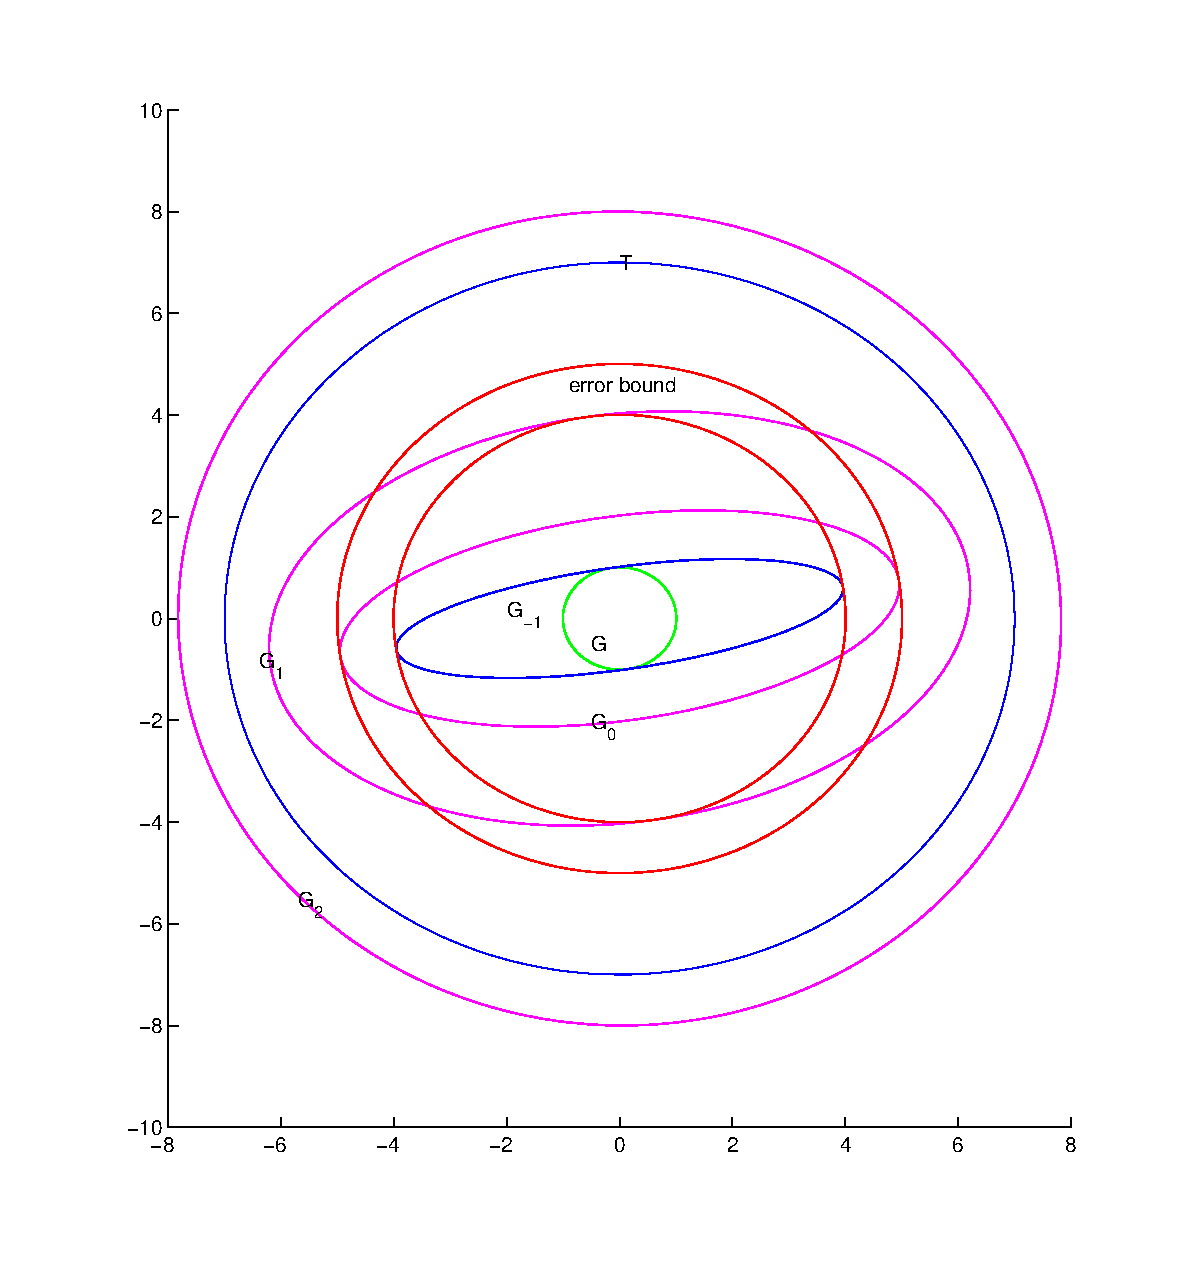
\includegraphics[width = 0.8\textwidth, height = 0.5\textheight]{sys.eps}
\end{center}
\caption{Иллюстрация взаимного расположения множеств ошибок в $\mathbb{R}^2$.}
%\end{multicols}
\end{figure}


=======
>>>>>>> minor revisions of measure concentration

\begin{equation*}
\begin{split}
&G_0 = (I-A)^{-1}G,\\
&G_m = A^{-m}G_0. 
\end{split}
\end{equation*} 
%Множества проиллюстрированы в Рис. \ref{krasn}.


%\begin{figure}[h]
%\begin{center}
%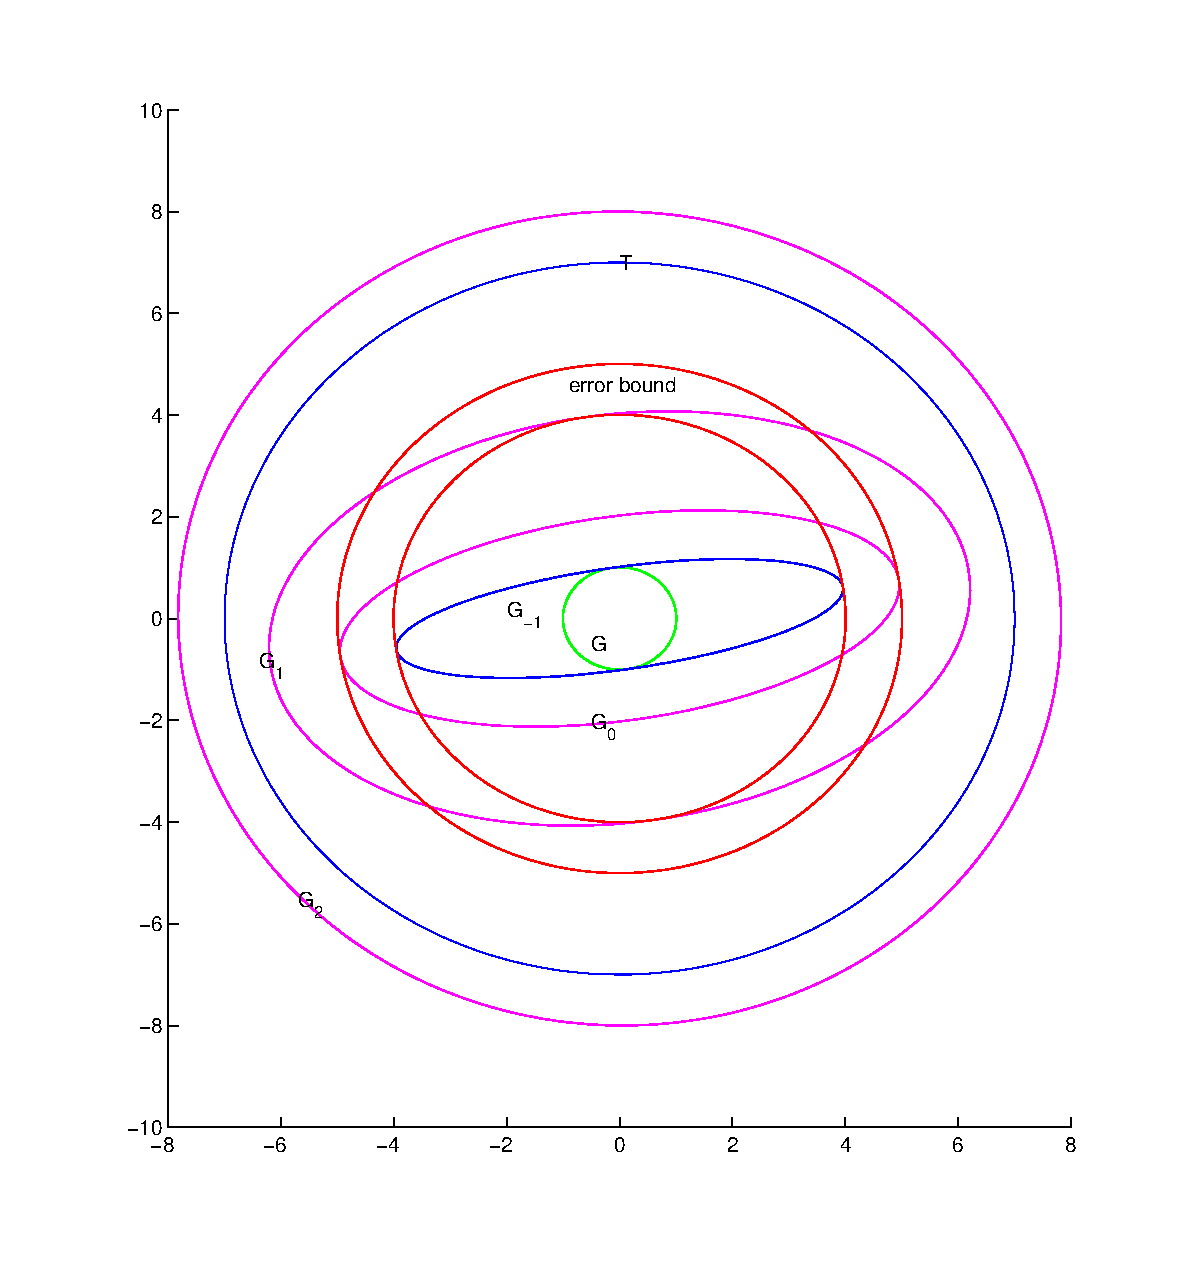
\includegraphics[width = 0.8\textwidth, height = 0.5\textheight]{sys.eps}
%\end{center}
%\caption{Иллюстрация взаимного расположения множеств ошибок в $\mathbb{R}^2$.}
%\label{krasn}
%\end{multicols}
%\end{figure}
\end{remark}

\subsection{Неравенства концентрации для сумм случайных величин ---  неравенства Чернова, Хевдинга, Бернштейна, Азумы}

%По мотивам лекции Голубева, обзора Лугоши.

%\begin{enumerate}
%\item
\begin{problem}[Неравенство  Чернова]

Доказать, что неравенство Чернова для неотрицательной случайной величины $X$
\begin{equation*}
\mathbf{P}\{ X >t\}\leq \inf_{s>0}\mathbf{E}\exp(sX-st)
\end{equation*}
 дает более завышенную границу по сравнению с моментной границей
\begin{equation*}
\mathbf{P}\{ X >t\}\leq \min_{q>0}\mathbf{E}[X^q]t^{-q},
\end{equation*}
 то есть 
\begin{equation*}
\min_q\mathbf{E}[X^q]t^{-q}\leq \inf_{s>0}\mathbf{E}\big[\text{e}^{s(X-t)}\bigl]
\end{equation*}
\end{problem}

\begin{remark} Использовать следствие из неравенства Маркова: для монотонной возрастающей неотрицаиельной функции $\phi(\cdot)$ и произвольной неотрицательной случайной величины $X$ верно
\begin{equation*}
\mathbf{P}\{\phi(X)\geq \phi(t)\}\leq \frac{\mathbf{E}\phi(X)}{\phi(X)}.
\end{equation*}
\end{remark}

%\item 
%\begin{problem}[Неравенство Чернова для суммы случайных величин]

%\end{problem}

<<<<<<< HEAD
%\item 
\begin{problem}[Лемма Хефдинга] Пусть $X$--- случайная величина, такая что $\mathbf{E}X =0$, $a\leq X\leq b$. Тогда для $s>0$ верно
\begin{equation*}
\mathbf{E}\exp(s X)\leq \exp\bigg[\frac{s^2(b-a)^2}{8}\biggr]
=======
%\item
\begin{problem}
\textbf{ЛЕММА.}\textsl{
Пусть $\xi_t$ ~--- гауссовские случайные величины с нулевым средним и $\mathbf{E}\xi_t^2 = \sigma^2_t\leq\sigma$. Тогда 
\begin{equation*}
\mathbf{E}\max_{t\in T}\xi_t \leq \sqrt{2\sigma^2\log(n)},
>>>>>>> minor revisions of measure concentration
\end{equation*}
здесь $n = \#T$~--- число элементов $T$.}

<<<<<<< HEAD
\begin{remark}
Использовать выпуклость экспоненты, для $a\leq x\leq b$

\begin{equation*}
\text{e}^{sx} \leq \frac{x-a}{b-a} \text{e}^{sb}+\frac{b-x}{b-a}\text{e}^{sa} 
\end{equation*}

Получить 

\begin{equation*}
\mathbf{E}\text{e}^{sx} \leq \text{e}^{\phi(u)}
\end{equation*}

где $u = s(b-a)$, $\phi(u) = -pu+\log(1-p+p\text{e}^u)$, $p = -a/(b-a)$.
Найти $\phi^{\prime\prime}(u)$,   $\phi(0)$, $\phi^{\prime}(0)$.

=======
\textbf{Доказательство.}  Для любого $\lambda>0$
\begin{equation*}
\max_{t\in T} \xi_t = \lambda^{-1}\log\big[\max_{t\in T} \rm e^{\lambda \xi_t}\bigr]\leq \lambda^{-1}\log\big[\sum_{t\in T}\rm e^{\lambda \xi_t}\bigr].
\end{equation*}
Воспользуемся далее неравенством Йенсена: если $f(\cdot)$ вогнутая функция, 
то
$
\mathbf{E}f(\xi)\leq f(\mathbf{E}\xi).
$
Имеем
\begin{equation*}
\begin{split}
\mathbf{E}\max_{t\in T} \xi_t \leq& \lambda^{-1}\log\big[\sum_{t\in T}\mathbf{E}\exp(\lambda \xi_t)\bigr]\\ &\leq \lambda^{-1}\log\big[ n \exp(\lambda^2 \sigma^2/2)\bigr] = \frac{\log(n)}{\lambda} + \frac{\sigma^2\lambda}{2}.
\end{split}
\end{equation*}


Поскольку это неравенство справедливо для любого $\lambda$, то чтобы улучшить верхнюю границу, минимизируем ее по $\lambda$. Находим 
\begin{equation*}
 -\frac{\log(n)}{\lambda^2} + \frac{\sigma^2}{2} = 0, \quad \lambda = \sqrt{\frac{2\log(n)}{\sigma^2}}.
\end{equation*}
Поэтому
\begin{equation*}
\mathbf{E}\max_{t\in T} \xi_t  \leq \log(n) \sqrt{\frac{\sigma^2}{2\log(n)}}+ \sqrt{\sigma^2{\log(n)/2}} = \sqrt{2\log(n)\sigma^2}. 
\end{equation*}
$\blacktriangle$

Наша задача ~--- вычислить
\begin{equation*}
\mathbf{E}\max_{t\in T}\xi_t.
\end{equation*}
Попробуем понять, насколько сложна эта задача. Именно, попробуем ответить на вопрос: насколько эта задача сложнее вычисления 
\begin{equation*}
\mathbf{E}\sum_{t\in T} \xi'_t = \sum_{t\in T}\mathbf{E}\xi'_t,
\end{equation*}
где $\xi'_t$ некоторый набор другиx с. в.
Основная идея доказательства: если случайные величины $\xi'_t>0$ имеют тяжелые хвосты, то 
\begin{equation*}
\max_{t\in T} \xi'_t \asymp \sum_{t\in T}\xi'_t.
\end{equation*}

\end{problem}
 
\begin{problem}[Лемма Хефдинга] Пусть $X$--- случайная величина, такая что $\mathbf{E}X =0$, $a\leq X\leq b$. Тогда для $s>0$ верно
\begin{equation*}
\mathbf{E}\exp(s X)\leq \exp\bigg[\frac{s^2(b-a)^2}{8}\biggr]
\end{equation*}
\end{problem}

\begin{remark}
Использовать выпуклость экспоненты, для $a\leq x\leq b$

\begin{equation*}
\text{e}^{sx} \leq \frac{x-a}{b-a} \text{e}^{sb}+\frac{b-x}{b-a}\text{e}^{sa} 
\end{equation*}

Получить 

\begin{equation*}
\mathbf{E}\text{e}^{sx} \leq \text{e}^{\phi(u)}
\end{equation*}

где $u = s(b-a)$, $\phi(u) = -pu+\log(1-p+p\text{e}^u)$, $p = -a/(b-a)$.
Найти $\phi^{\prime\prime}(u)$,   $\phi(0)$, $\phi^{\prime}(0)$.

>>>>>>> minor revisions of measure concentration
Показать, что 
\begin{equation*}
\phi^{\prime\prime}(u)\leq \frac{1}{4}.
\end{equation*}

Используя формулу Тейлора, получить  
\begin{equation*}
\phi(u) \leq \frac{u^2}{8}\leq \frac{s^2(b-a)^2}{8}.
\end{equation*}
\end{remark}

\begin{problem}[Теорема Хефдинга] Пусть $\xi_t$, $t\in T$ ~--- независимые случайные величины, такие что $\xi_t\in[a,b]$. Тогда
\begin{equation*}
\mathbf{P}\bigg\{\bigg|\frac{1}{n}\sum_{t\in T}\big(\xi_t-\mathbf{E}\xi_t\bigr)\biggr|\geq x\biggr\}\leq 2\exp\bigg\{-\frac{2nx^2}{(b-a)^2}\biggr\}.
\end{equation*}
\end{problem}
\begin{remark}
Ввести случайную величину $\xi = \frac{1}{n}\sum_{i=1}^n(\xi_i-\mathbf{E}\xi_i)$.
Воспользоваться неравеством Чернова и леммой Хевдинга для $\xi$, чтобы получить
\begin{equation*}
\mathbf{P}\{\xi>x\}\leq \exp\bigg\{\min_{\lambda}\bigg[-\lambda x + \frac{\lambda^2}{8}\frac{(b-a)^2}{n}\biggr]\biggr\}.
\end{equation*}
Затем найти оптимальное $\lambda$.  Аналогичное неравенство справедливо для $-\xi$.
\end{remark}

\begin{problem}[Неравенство Беннетта]
Пусть $X_1,\dots, X_n$ независимые центрированные ограниченные случайные величины, такие, что с вероятностью $1$ выполнено $|X_i|\leq c$.
Пусть $\sigma^2 = \sum_{i=1}^n\text{Var}\{X_i\}$.
 Тогда для любого $t>0$ 
\begin{equation*}
\mathbf{P}\bigg\{\sum_{i=1}^n X_i>t\biggr\}\leq \exp\bigg(-\frac{n\sigma^2}{c^2}h\bigg(\frac{ct}{n\sigma^2}\biggr)\biggr),
\end{equation*}
где $h(u) = (1+u)\log(1+u)-u$ для $u\geq 0$.
\end{problem}
\begin{remark}
Введем $\sigma_i^2 = \mathbf{E}[X_i^r]$ и $F_i = \sum_{r=2}^{\infty}\frac{s^{r-2}\mathbf{E}[X_i^r]}{r!\sigma_i^2}$.
Используя разложение для ряда Тейлора $\exp(sX)$, показать, что 
\begin{equation*}
\mathbf{E}[e^{sX_i}]\leq \exp(s^2\sigma^2_iF_i).
\end{equation*}

Из ограниченности  $X_i$ получить оценку
\begin{equation*}
F_i\leq \frac{\exp(sc)-1-sc}{(sc)^2}.
\end{equation*} 
Далее воспользоваться неравенством Чернова для $X_i$ и минимизировать правую часть в неравенстве Чернова по $s$.
\end{remark}

\begin{problem}[Неравенство Бернштейна]
При выполнении условий предыдущей теоремы для любого  $\epsilon>0$ верно 
\begin{equation*}
\mathbf{P}\bigg\{\frac{1}{n}\sum_{i=1}^n X_i>\epsilon\biggr\}\leq \exp\bigg(-\frac{n\epsilon^2}{2\sigma^2+2c\epsilon/3}\biggr).
\end{equation*}
\end{problem}

\begin{remark} 
Показать, что верно элементарное неравенство 
\begin{equation*}
h(u)\geq \frac{u^2}{2+2u/3}
\end{equation*}
и использовать неравенство Беннетта.
\end{remark}
%\end{enumerate}

\begin{problem} Пусть $Y$ случайная величина,  $Y\in [-1,+1]$ и $\mathbf{E}[Y]=0$. Тогда для любого $t\geq 0$ верно 
\begin{equation*}
\mathbf{E}[\exp(tY)]\leq \exp(t^2/2).
\end{equation*}
\end{problem}

\begin{remark}
Использовать выпуклость $\exp(tx)$, а именно для $x\in[-1,1]$ верно.
\begin{equation*}
\text{e}^{tx}\leq \frac{1}{2}(1+x)\text{e}^{t} +\frac{1}{2}(1-x)\text{e}^{-t}
\end{equation*}
Подсчитать оценку математического ожидания $\mathbf{E}[\text{e}^{tY}]$ используя разложение экспоненты в ряд Тейлора и элементарный факт $(2n)!>2^nn!$.  
\end{remark}

\begin{problem}[Мартингальное неравенство Азумы-Хевдинга]

Пусть $\{X_i\}_{i=0}^{\infty}$ мартингал по отношению к фильтрации $\{\mathcal{F}_i\}$, пусть $Y_i = X_i-X_{i-1}$ соответствующая последовательность приращений. Тогда, если существуют такие $c_i>0$, что $|Y_i|\leq c_i$ для всех $i$, то 
\begin{equation*}
\mathbf{P}\{\sup_{n\geq m} |X_n-X_0|\geq t\}\leq 2\exp\bigg\{\frac{-t^2}{2\sum_{i=1}^{m}c^2_i}\biggl\}
\end{equation*}
\end{problem}

\begin{remark} Способы доказательства неравенства Азумы-Хевдинга. 
\medskip
\begin{enumerate}

\item \textit{Первый способ доказательства использует теорему Дуба (см. введение).} 

\textbf{TODO}


\item \textit{Второй способ для доказательства не равномерного варианта теоремы использует результат задачи 12.}

Показать, что 
\begin{equation*}
\mathbf{E}\exp(sY_1+\dots+ sY_m) = \mathbf{E}\big[\exp(sY_1+\dots+sY_{m-1})\mathbf{E}[\exp(sY_m)|\mathcal{F}_{m-1}]\bigl] 
\end{equation*}
записать неравенство Чернова

\begin{equation*}
\mathbf{P}[Y_1+\dots+Y_m>t]\leq \exp\big[-st+\sum_{i=1}^mc^2_i s^2/2\bigr].
\end{equation*}
Остается оценить $s$ из минимизации правой части.
\end{enumerate}

\end{remark}



\begin{problem}
<<<<<<< HEAD
Что можно сказать о том, как соотносятся между собой неравенство Бернштейна и Хевдинга? Рассмотреть Неравенство Бернштейна в случаях, когда $\sigma^2>\epsilon$ и когда $\sigma^2<\epsilon$. Что можно сказать про достижимость неравенства Бернштейна? 
=======
Что можно сказать о том, как соотносятся между собой неравенство Бернштейна и Хевдинга? Рассмотреть неравенство Бернштейна в случаях, когда $\sigma^2>\epsilon$ и когда $\sigma^2>\epsilon$. Что можно сказать про достижимость неравенства Бернштейна? 
>>>>>>> minor revisions of measure concentration
\begin{remark}
Рассмотреть предельную теорему Пуассона.
\end{remark}
\end{problem}

\subsection{Неравенства концентрации меры для функционалов от случайных величин.}
\medskip

\begin{problem}[Неравенство Эфрона-Стейна]
Пусть $X'_1,\dots,X'_n$ ~--- независимые копии $X_1,\dots,X_n$ и 
\begin{equation*}
Z'_i = g(X_1,\dots, X'_i,\dots,X_n).
\end{equation*}
Тогда верно неравенство 
\begin{equation*}
\text{Var}(Z)\leq \frac{1}{2}\sum_{i=1}^{n}\mathbf{E}[(Z-Z'_i)^2].
\end{equation*}
\end{problem}
\begin{remark}
 
Пусть $X_1,\dots, X_n$, произвольные независимые (не обязательно одинаково распределенные случайные величины) принимающие значения из $\mathcal{X}$ и пусть  $g: \mathcal{X}^n\to \mathbf{R}$ измеримая функция $n$ переменных. Показать, что для случайной величины $Z = g(X_1,\dots,X_n)$ верно 
\begin{equation*}
\text{Var}(Z) \leq \sum_{i=1}^n \mathbf{E}\big[ (Z-\mathbf{E}_iZ)^2\bigl],
\end{equation*}
где $\mathbf{E}_iZ = \mathbf{E}[Z|X_1,\dots,X_{i-1},X_{i+1},\dots,X_n]$.
\end{remark}
\begin{problem}[Случай функций с ограниченными  разностями]
Функция $g: \mathcal{X}^n\to \mathbf{R}$ является функцией с ограниченными разностями, если для некоторых $c_i,$  $1\leq i\leq n$.
\begin{equation*}
\sup_{x_1,\dots,x_n;\, x'_i\in\mathcal{X}} |g(x_1,\dots,x_n)-g(x_1,\dots,x_{i-1},x'_i,x_{i+1},\dots,x_{i+1},\dots,x_n)|\leq c_i. 
\end{equation*}
Выпишите неравенство Эфрона-Стейна для случая функций с ограниченными разностями.
\end{problem}
\medskip

\subsection{Вероятности больших уклонений}


Рассматриваются вероятности $\mathbf{P}\biggl\{\Bigl|\sum_{i=1}^n\xi_i -\sum_{i=1}^m m_i\Bigr|\geq t\biggr\}$ для последовательности независимых величин $\xi_1,\xi_2,\dots$ с математическими ожиданиями $m_i = \mathbf{E} \xi_i$ и $\text{Var} \xi_i = d$. 
Если использовать для оценки этой вероятности неравенство Чебышева, то при $t = c\sqrt{n}$ и $t=cn$, где $c$~--- некоторая постоянная, получается разный порядок сходимости вероятности. В отличае от первого случая, оценка при $t=cn$ является очень грубой. 

\medskip 

Введем ряд обозначений
\begin{equation*}
\mathbf{P}_{n,c} = \mathbf{P}\biggl\{\Bigl|\sum_{i=1}^n\xi_i -\sum_{i=1}^m m_i\Bigr|\geq cn\biggr\},
\end{equation*}
\begin{equation*}
R(\lambda)=\int_{-\infty}^{\infty}\text{e}^{\lambda x}\,d F(x),
\end{equation*}
\begin{equation*}
m(\lambda) = \frac{R^{\prime}(\lambda)}{R(\lambda)}.
\end{equation*}

\medskip

Оказывается, что при условии 
\begin{equation}
R(\lambda)<\infty
\label{condition.R}
\end{equation}
верна более точная оценка 
\begin{equation*}
\lim_{n\to\infty}\frac{1}{n}\ln \mathbf{P}_{n,c} =\ln r(\lambda_0),
\end{equation*}
где 
\begin{equation*}
r(\lambda_0) = \text{e}^{-\lambda_0 c}R(\lambda_0),
\end{equation*}
значение $\lambda_0$ удовлетворяет условию  $m(\lambda_0) = c$.

\medskip

Для того, чтобы это показать, докажите следующие утверждения.

\begin{problem}
Будем говорить, что $M^{+}$ есть верхний предел по вероятности случайной величины $\xi$, если $\mathbf{P}\{\xi>M^{+}\} = 0$ и $\mathbf{P}\{M^{+}-\epsilon\leq\xi\leq M^{+}\}>0$ для каждого  $\epsilon>0$. Нижний предел по вероятности можно определить тем же образом. Если $\mathbf{P}\{\xi>M\}>0$, ($\mathbf{P}\{\xi<M\}>0$) для всякого $M$, то $M^{+}=\infty$ ($M^{-}=-\infty$). Во всех остальных случаях $M^{+}$ и $M^{-}$ конечны.
Показать, что при условии \eqref{condition.R} 
функция $m(\lambda)$ имеет следующие пределы
\begin{equation*}
\lim_{\lambda\to\infty}m(\lambda) = M^{+},\quad \lim_{\lambda\to -\infty} = M^{-}.
\end{equation*}
\end{problem}
\begin{remark}

<<<<<<< HEAD
\textbf{TODO}

\end{remark}
\begin{problem}
Имеет место неравенство 
\begin{equation*}
\mathbf{P}_{n,c} \leq B_n(R(\lambda_0))\text{e}^{-\lambda_0c})^n,\quad\text{где} \lim_{n\to\infty}B_n=\frac{1}{2}.
\end{equation*}
\end{problem}
\begin{remark}

\textbf{TODO}

\end{remark}
\begin{problem}
Для всякого $b>0$ существует такое $p(b,\lambda_0)>0$, что 
\begin{equation*}
\mathbf{P}_{n,c} \geq (R(\lambda_0))\text{e}^{-\lambda_0c})^n\text{e}^{-\lambda_0 b \sqrt{n}} p_n, 
\end{equation*}
причем $\lim_{n\to\infty}p_n = p(b,\lambda_0)$.
\end{problem}
\begin{remark}
\textbf{TODO}
=======
\textbf{TODO}

\end{remark}
\begin{problem}
Имеет место неравенство 
\begin{equation*}
\mathbf{P}_{n,c} \leq B_n(R(\lambda_0)\text{e}^{-\lambda_0c})^n,\quad\text{где} \lim_{n\to\infty}B_n=\frac{1}{2}.
\end{equation*}
\end{problem}
\begin{remark}

\textbf{TODO}

\end{remark}
\begin{problem}
Для всякого $b>0$ существует такое $p(b,\lambda_0)>0$, что 
\begin{equation*}
\mathbf{P}_{n,c} \geq (R(\lambda_0)\text{e}^{-\lambda_0c})^n\text{e}^{-\lambda_0 b \sqrt{n}} p_n, 
\end{equation*}
причем $\lim_{n\to\infty}p_n = p(b,\lambda_0)$.
\end{problem}
\begin{remark}
\textbf{TODO}
>>>>>>> minor revisions of measure concentration
\end{remark}
%\begin{problem}[Задача о среднем функции в смысле Леви --- про концентрацию меры на сфере вокруг медианного значения "хорошей" функции]
%\end{problem}
%\subsection{Изопериметрические неравенства Талаграна(?)}


\section{Три кита математической статистики}

\section{Разные задачи}

\begin{problem}
(Распределения канторовского типа).

Рассмотрим в $\sum _{k=1}^{\infty }2^{-k} X_{k}  $, где $X_{k} $ - взаимно независимые с.в., имеющие распределение Бернулли с параметром ${1\mathord{\left/ {\vphantom {1 2}} \right. \kern-\nulldelimiterspace} 2} $, сумму слагаемых с четными номерами, или, что с точностью до множителя 3 (в дальнейшем потребуется для удобства) есть $Y=3\sum _{s=1}^{\infty }4^{-s} X_{s}  $. Покажите, что функция распределения $F(x)=P\left\{Y\le x\right\}$ является сингулярной (когда не оговаривается относительно какой меры, подразумевается, что относительно меры Лебега).


\begin{ordre}
Можно рассматривать $Y$ как выигрыш игрока, который получает $3\cdot 4^{-k} $, когда $k$-е бросание симметричной монеты дает в результате решку. Ясно, что полный выигрыш лежит между 0 и $3\left(4^{-1} +4^{-2} +\ldots \right)=1$. Если первое подбрасывание монеты привело к решке, то полный выигрыш $\ge {3\mathord{\left/ {\vphantom {3 4}} \right. \kern-\nulldelimiterspace} 4} $, тогда как в противоположном случае $Y\le 3\left(4^{-2} +4^{-3} +\ldots \right)=4^{-1} $. То есть неравенство ${1\mathord{\left/ {\vphantom {1 4}} \right. \kern-\nulldelimiterspace} 4} <Y<{3\mathord{\left/ {\vphantom {3 4}} \right. \kern-\nulldelimiterspace} 4} $ не может быть осуществлено ни при каких обстоятельствах, значит $F(x)={1\mathord{\left/ {\vphantom {1 2}} \right. \kern-\nulldelimiterspace} 2} $ в интервале $x\in \left({1\mathord{\left/ {\vphantom {1 4}} \right. \kern-\nulldelimiterspace} 4} ,{3\mathord{\left/ {\vphantom {3 4}} \right. \kern-\nulldelimiterspace} 4} \right)$. Чтобы определить, как ведет себя функция распределения на интервале $x\in \left(0,{1\mathord{\left/ {\vphantom {1 4}} \right. \kern-\nulldelimiterspace} 4} \right)$, покажите, что на этом интервале график отличается только преобразованием подобия $F(x)={1\mathord{\left/ {\vphantom {1 2}} \right. \kern-\nulldelimiterspace} 2} F(4x)$.
\end{ordre}

\begin{remark}
Пример, когда свертка двух сингулярных распределений имеет непрерывную плотность: с.в. $X=\sum _{k=1}^{\infty }2^{-k} X_{k}  $ имеет равномерное распределение на $\left(0;1\right)$. Обозначим сумму членов ряда с четными и нечетными номерами через $U$ и $V$ соответственно. Ясно, что $U$ и $2V$ имеют одинаковое распределение и их распределение относится к канторовскому типу.
\end{remark}

\end{problem}


\begin{problem}
Напомним, что сингулярными мерами называются меры, функции распределения $F(x)$ которых непрерывны, но точки их роста ($x$ -- точка роста $F(x)$, если для любого $\varepsilon >0$ выполняется: $F(x+\varepsilon )-F(x+\varepsilon )>0$) образуют множество нулевой меры Лебега. Покажите, что мера, соответствующая функции Кантора, сингулярна по отношению к мере Лебега.

\end{problem}


\begin{problem} (повторяется)
Доказать неравенство Чернова:

\[P\left\{\sum _{i=1}^{n}X_{i} >(p+t)n \right\}\le \exp \left\{nH\left(\left\{p+t,q-t\right\},\left\{p,q\right\}\right)\right\},\quad 0\le t\le q,\] 
где $X_{i} $, $i=1,...,n$ - независимые случайные величины, имеющие распределение Бернулли:
\[X_{i} =\left\{\begin{array}{cc} {1,} & {p,} \\ {0,} & {q=1-p;} \end{array}\right. \] 
$H\left(P,Q\right)=\sum _{j=1}^{m}-P_{j} \log \frac{P_{j} }{Q_{j} }  $ - относительное энтропийное «расстояние» между двумя (дискретными) распределениями вероятностей $P=\left(P_{1} ,\ldots ,P_{m} \right)$ и $Q=\left(Q_{1} ,\ldots ,Q_{m} \right)$ на пространстве элементарных исходов размера $m$.

\begin{ordre}
 
Воспользуйтесь техникой получения неравенства Азумы, а именно 

\noindent \textbf{а)} перейдите к положительной случайной величине $e^{\lambda \sum _{i=1}^{n}X_{i}  } $($\lambda >0$ - некий параметр). В теории вероятностей функция $\varphi _{Y} (\lambda )=E\left[e^{\lambda Y} \right]$называется производящей функции моментов случайной величины $Y$, так как при разложении в ряд Тейлора $\varphi _{Y} (\lambda )=E\left[e^{\lambda Y} \right]=E\left[\sum _{i=0}^{\infty }\frac{\lambda ^{i} }{i!} Y^{i}  \right]=\sum _{i=0}^{\infty }\frac{\lambda ^{i} }{i!} E\left[Y^{i} \right] $, где $E\left[Y^{i} \right]$ - \textit{i}-ый момент случайной величины $Y$.

\noindent \textbf{б)} применив неравенство Маркова , получите $P\left\{\sum _{i=1}^{n}X_{i} > \; m\right\}=P\left\{e^{\lambda \sum _{i=1}^{n}X_{i}  } >e^{m} \right\}\le \left(\frac{pe^{\lambda } +q}{e^{\lambda (p+t)} } \right)^{n} $ с параметризацией $m=(p+t)n$.

\noindent \textbf{в)} подобрав оптимальное значение ($\frac{pe^{\lambda } +q}{e^{\lambda (p+t)} } \to \mathop{\min }\limits_{\lambda } $), получите 

\[
P\left\{\sum _{i=1}^{n}X_{i} >(p+t)n \right\}\le \left(\left(\frac{p}{p+t} \right)^{p+t} \left(\frac{q}{q-t} \right)^{q-t} \right)^{n} 
\]
\[
= \exp \left\{n\left[-(p+t)\ln \frac{p+t}{p} -(q-t)\ln \frac{q-t}{q} \right]\right\}.
\] 


\end{ordre}

\begin{remark}
C точки зрения математической статистики 

\[
H\left(\left\{p+t,q-t\right\},\left\{p,q\right\}\right)=-(p+t)\ln \frac{p+t}{p} -(q-t)\ln \frac{q-t}{q} 
\]

-энтропийное расстояние между апостериорным (полученным после эксперимента) распределением $\left\{p+t,q-t\right\}$и априорным $\left\{p,q\right\}$. Таким образом, «граница» Чернова уменьшается экспоненциально с показателем равным n-кратному энтропийному расстоянию между апостериорным и априорным распределением вероятностей.\textbf{}

\noindent Более удобная запись «границы» Чернова:
\[P\left\{\sum _{i=1}^{n}X_{i} >(p+t)n \right\}\le \exp \left\{-\frac{2t^{2} }{n} \right\},\] 
так как для функции $f(t)=(p+t)\ln \frac{p+t}{p} +(q-t)\ln \frac{q-t}{q} $ имеем $f(0)=f'(0)=0$, $f''(t)=\frac{1}{(p+t)(q-t)} \ge 4$ для любого $0\le t\le q$, значит разложение Тейлора 
\[f(t)=f(0)+f'(0)t+f''(\xi )\frac{t^{2} }{2!} \ge 2t^{2} ,\quad 0<\xi <t.\]

\end{remark}

\end{problem}

\begin{problem}

Доказать оценку для больших уклонений в Бернуллиевской модели:
\[X_{i} =\left\{\begin{array}{cc} {1,} & {p,} \\ {0,} & {q=1-p;} \end{array}\right. \] 
$P\left\{\sum _{i=1}^{n}X_{i} =\left[\alpha n\right] \right\}\sim \frac{1}{\sqrt{2\pi \alpha (1-\alpha )} } \exp \left\{nH(\{ p,1-p\} ,\{ \alpha ,1-\alpha \} )\right\}$, $0<\alpha <1$ и $\alpha \ne p,$

\noindent где $H\left(P,Q\right)=\sum _{j=1}^{m}-P_{j} \log \frac{P_{j} }{Q_{j} }  $ - относительное энтропийное «расстояние» между двумя (дискретными) распределениями вероятностей $P=\left(P_{1} ,\ldots ,P_{m} \right)$ и $Q=\left(Q_{1} ,\ldots ,Q_{m} \right)$ на пространстве элементарных исходов размера $m$.

\begin{ordre}

Напомним, что производящей функцией (п.ф.) некоторой целочисленной неотрицательной случайной величины (с.в.) $\xi $ называется $\varphi _{\xi } (z)=Ez^{\xi } =\sum _{j=0}^{\infty }P\left\{\xi =j\right\} z^{j} $. Зная распределение с.в. можно получить ее п.ф., и наоборот, задание п.ф. однозначно определяет ее распределение: (для этого можно воспользоваться теорией функций комплексного переменного -- теоремой Коши -- для определения коэффициентов в разложении аналитической функции в ряд Лорана) $P\left\{\xi =k\right\}=\left[z^{k} \right]\varphi _{\xi } (z)=\frac{1}{2\pi i} \oint _{\left|z\right|=1}\frac{\varphi _{\xi } (z)}{z^{k+1} } dz $. Также следует напомнить, что п.ф. для суммы независимых с.в. справедливо $\varphi _{\sum _{i=1}^{n}X_{i}  } (z)=Ez^{\sum _{i=1}^{n}X_{i}  } =E\left[\prod _{i=1}^{n}z^{X_{i} }  \right]=\prod _{i=1}^{n}Ez^{X_{i} }  =\prod _{i=1}^{n}\varphi _{X_{i} } (z) $. Таким образом, в данной задаче $P\left\{\sum _{i=1}^{n}X_{i} =\left[\alpha n\right] \right\}=\left[z^{\left[\alpha n\right]} \right]\varphi _{\sum _{i=1}^{n}X_{i}  } (z)=\frac{1}{2\pi i} \oint _{\left|z\right|=\rho }\frac{\left(pz+q\right)^{n} }{z^{\left[\alpha n\right]+1} } dz $,\textbf{ }последний интеграл можно оценить с помощью методе перевала: перейдя к полярным координатам $z=\rho e^{i\theta } $ и сделав замену, получим:\textbf{}
\[\frac{1}{2\pi i} \oint _{\left|z\right|=1}\frac{\left(pz+q\right)^{n} }{z^{\left[\alpha n\right]+1} } dz =\frac{1}{2\pi } \int _{-\pi }^{\pi }e^{nf\left(\rho e^{i\theta } \right)} d\theta  ,\] 
где $f(z)=\ln \left(pz+q\right)-\left(\alpha -\frac{\varepsilon _{n} }{n} \right)\ln z$ ($\left[\alpha n\right]=\alpha n-\varepsilon _{n} $). Далее, нужно найти седловую точку и ограничиться интегрированием по её малой окрестности, разлагая подынтегральное выражение в ряд Тейлора.

\end{ordre}

\end{problem} % разное

\newpage

% Требование РИО "Литература" вместо "Список литературы"
\renewcommand\refname{Литература}
% В самом списке 1. вместо [1]
\makeatletter
\renewcommand{\@biblabel}[1]{#1.}
\makeatother

\begin{thebibliography} {20}

\bibitem{1} 
Боровков А.А. Теория вероятностей. – М.: Наука, 1986. –: 352 с. (и более поздние издания)

\bibitem{2} 
Гнеденко Б.В. Курс теории вероятностей. – М: Наука, 1988. – 446 с. (и более поздние издания)

\bibitem{3}
Колмогоров А.Н. Основные понятия теории вероятностей. – М.: Наука. 1974. – 120 с.

\bibitem{4} 
Ширяев А.Н. Вероятность. – М.: Наука, 1989. – 640 с. (и более поздние издания)

\bibitem{5} 
Натан А.А., Горбачев О.Г., Гуз С.А. Теория вероятностей: Учеб. пособие. – М.: МЗ Пресс – МФТИ, 2007. – 253 с.

\bibitem{6} 
Розанов Ю.А. Лекции по теории вероятностей. - Долгопрудный: Издательский дом “Интеллект”, 2008. – 136 с.

\bibitem{7} 
Ширяев А.Н. Задачи по теории вероятностей. – М.: МЦНМО, 2006. – 416 с.

\bibitem{8} 
Гмурман В.Е. Руководство к решению задач по теории вероятностей и математической статистике. – М.: Высшая школа, 1979. – 400 с. (и более поздние издания)

\bibitem{9} 
Зубков А.М., Севастьянов Б.А., Чистяков В.П. Сборник задач по теории вероятностей. – М.: Наука, 1989. – 320 с.

\bibitem{10} 
Прохоров А.В., Ушаков В.Г., Ушаков Н.Г. Задачи по теории вероятностей. Основные понятия. Предельные теоремы. Случайные процессы. – М.: Наука, 1986. – 328 с.

\bibitem{11} 
Стоянов Й. Контрпримеры в теории вероятностей. – М.: Факториал, 1999. – 288 с.

\bibitem{12} 
Секей Г. Парадоксы в теории вероятностей и математической статистике. – М.: РХД, 2003. – 272 с.

\bibitem{13} 
Flajolet P., Sedgewick R. Analytic combinatorics. Cambridge University Press, 2008. 

\bibitem{14} 
Ledoux M. Concentration of measure phenomenon, Providence, RI, Amer. Math. Soc., 2001 (Math. Surveys Monogr. V. 89)

\bibitem{15} 
Алон Н., Спенсер Дж. Вероятностный метод. Бином, 2006.

\bibitem{16} 
Кендалл М., Моран П. Геометрические вероятности. М.: Наука, 1972.

\bibitem{17} 
Motwani R., Raghavan P. Randomized algorithms. Cambridge Univ. Press, 1995.

\bibitem{18} 
Cover T.M., Thomas J.A. Elements of Information theory. Wiley-Interscience, 2006. 

\bibitem{19} 
Durrett R. Probability: Theory and Examples. Cambridge Univ. Press, 2010.

\bibitem{20} 
Кац М. Вероятность и смежные вопросы в физике. М.: Мир, 1965.


\end{thebibliography}




\end{document}
